% GENERATED by scripts/make_tmlr_manuscript.py -- do not edit by hand.
\documentclass[10pt]{article}
\usepackage{tmlr}
\usepackage{hyperref}
\usepackage{url}
\usepackage{amsmath}
\usepackage{amssymb}
\usepackage{amsthm}
\usepackage{graphicx}
\usepackage{booktabs}
\usepackage{tabularx}
\usepackage{seqsplit}
\usepackage[section]{placeins}

\newtheorem{proposition}{Proposition}[section]
\newtheorem{theorem}{Theorem}[section]
\newtheorem{lemma}{Lemma}[section]
\newtheorem{corollary}{Corollary}[section]

% Generated by scripts/create_results_macros.py from outputs/*.json -- do not hand-edit.
\def\TracksTableRows{B --- GSM8K, homog. & 40/40 & 100.0 & 100.0 & 100.0 & -- \\
B$'$ --- GSM8K, heterog. & 40/40 & \textbf{100.0} & \textbf{100.0} & 95.0 & -- \\
C --- MATH L5, homog. & 134/134 & 89.6 & \textbf{91.0} & 89.6 & 90.3 \\
C$'$ --- MATH L5, heterog. & 134/134 & 88.1 & \textbf{90.3} & 79.1 & 79.9 \\
D --- AIME 2026, homog. & 30/30 & 80.0 & 86.7 & \textbf{90.0} & 83.3 \\
D$'$ --- AIME 2026, heterog. & 30/30 & 86.7 & \textbf{93.3} & 63.3 & 90.0 \\
E --- GPQA Diamond, homog. & 198/198 & 75.3 & \textbf{78.8} & \textbf{78.8} & 78.3 \\
E$'$ --- GPQA Diamond, heterog. & 198/198 & 74.7 & 77.3 & \textbf{79.3} & 72.7 \\
F --- AIME 2025, homog. & 30/30 & 80.0 & \textbf{83.3} & 76.7 & 86.7 \\
G --- MMLU-Pro, homog. & 100/100 & 85.0 & \textbf{86.0} & \textbf{86.0} & 83.0 \\}
\def\PairedTableRows{B --- GSM8K, homog. & 0/0 & -- & 0/0 & -- & -- & -- \\
B$'$ --- GSM8K, heterog. & 0/2 & 0.500 & 0/2 & 0.500 & -- & -- \\
C --- MATH L5, homog. & 0/2 & 0.500 & 1/1 & 1.000 & 1/2 & 1.000 \\
C$'$ --- MATH L5, heterog. & 0/15 & $<$0.001 & 4/16 & 0.012 & 7/8 & 1.000 \\
D --- AIME 2026, homog. & 1/0 & 1.000 & 3/0 & 0.250 & 2/0 & 0.500 \\
D$'$ --- AIME 2026, heterog. & 0/9 & 0.004 & 0/7 & 0.016 & 1/9 & 0.021 \\
E --- GPQA Diamond, homog. & 6/6 & 1.000 & 13/6 & 0.167 & 9/8 & 1.000 \\
E$'$ --- GPQA Diamond, heterog. & 10/6 & 0.454 & 20/11 & 0.150 & 24/11 & 0.041 \\
F --- AIME 2025, homog. & 1/3 & 0.625 & 1/2 & 1.000 & 1/4 & 0.375 \\
G --- MMLU-Pro, homog. & 2/2 & 1.000 & 3/2 & 1.000 & 5/2 & 0.453 \\}
\def\HomogPooledN{532}
\def\HomogPooledB{10}
\def\HomogPooledC{13}
\def\HomogPooledP{$p=0.678$}
\def\TotalProblems{532}
\def\FigLabels{GSM8K,GSM8K-H,MATH5,MATH5-H,AIME,AIME-H,GPQA,GPQA-H,AIME25,MMLU-Pro}
\def\FigGRCoordinates{(GSM8K,100.0) (GSM8K-H,100.0) (MATH5,89.6) (MATH5-H,88.1) (AIME,80.0) (AIME-H,86.7) (GPQA,75.3) (GPQA-H,74.7) (AIME25,80.0) (MMLU-Pro,85.0)}
\def\FigSCCoordinates{(GSM8K,100.0) (GSM8K-H,100.0) (MATH5,91.0) (MATH5-H,90.3) (AIME,86.7) (AIME-H,93.3) (GPQA,78.8) (GPQA-H,77.3) (AIME25,83.3) (MMLU-Pro,86.0)}
\def\FigORCoordinates{(GSM8K,100.0) (GSM8K-H,95.0) (MATH5,89.6) (MATH5-H,79.1) (AIME,90.0) (AIME-H,63.3) (GPQA,78.8) (GPQA-H,79.3) (AIME25,76.7) (MMLU-Pro,86.0)}
\def\FigKYCoordinates{(MATH5,90.3) (MATH5-H,79.9) (AIME,83.3) (AIME-H,90.0) (GPQA,78.3) (GPQA-H,72.7) (AIME25,86.7) (MMLU-Pro,83.0)}
\def\HeteroPooledN{402}
\def\HeteroPooledB{10}
\def\HeteroPooledC{32}
\def\HeteroPooledP{$p<0.001$}
\def\ExtendedTableRows{C --- MATH L5, homog. & 132 & 90.9 & 92.4 & 2 & 89.6 & 91.0 \\
C$'$ --- MATH L5, heterog. & 131 & 79.4 & 90.8 & 3 & 79.1 & 90.3 \\
D --- AIME 2026, homog. & 24 & 95.8 & 91.7 & 6 & 90.0 & 86.7 \\
D$'$ --- AIME 2026, heterog. & 23 & 78.3 & 100.0 & 7 & 63.3 & 93.3 \\
E --- GPQA Diamond, homog. & 175 & 82.3 & 82.9 & 23 & 78.8 & 78.8 \\
E$'$ --- GPQA Diamond, heterog. & 163 & 85.3 & 82.8 & 35 & 79.3 & 77.3 \\
F --- AIME 2025, homog. & 24 & 87.5 & 95.8 & 6 & 76.7 & 83.3 \\
G --- MMLU-Pro, homog. & 94 & 88.3 & 88.3 & 6 & 86.0 & 86.0 \\}
\def\CoverageTableRows{B --- GSM8K, homog. & 40 & 40 & 0 & 0 & 0 & -- \\
B$'$ --- GSM8K, heterog. & 40 & 40 & 0 & 0 & 0 & 40 \\
C --- MATH L5, homog. & 134 & 134 & 0 & 0 & 0 & -- \\
C$'$ --- MATH L5, heterog. & 134 & 134 & 0 & 0 & 0 & 131 \\
D --- AIME 2026, homog. & 30 & 30 & 0 & 0 & 0 & -- \\
D$'$ --- AIME 2026, heterog. & 30 & 30 & 0 & 0 & 0 & 23 \\
E --- GPQA Diamond, homog. & 198 & 198 & 0 & 0 & 0 & -- \\
E$'$ --- GPQA Diamond, heterog. & 198 & 198 & 0 & 0 & 0 & 80 \\
F --- AIME 2025, homog. & 30 & 30 & 0 & 0 & 0 & -- \\
G --- MMLU-Pro, homog. & 100 & 100 & 0 & 0 & 0 & -- \\}
\def\KYTopOneN{854}
\def\KYTopOneDiffers{139}
\def\KYORwins{50}
\def\KYKYwins{44}
\def\NGSMh{40}
\def\TotGSMh{40}
\def\AccORGSMh{100.0}
\def\AccSCGSMh{100.0}
\def\AccGRGSMh{100.0}
\def\DiscGSMh{0}
\def\ORwinsGSMh{0}
\def\SCwinsGSMh{0}
\def\LegacyGSMh{0}
\def\NGSMx{40}
\def\TotGSMx{40}
\def\AccORGSMx{95.0}
\def\AccSCGSMx{100.0}
\def\AccGRGSMx{100.0}
\def\DiscGSMx{2}
\def\ORwinsGSMx{0}
\def\SCwinsGSMx{2}
\def\LegacyGSMx{40}
\def\NMATHh{134}
\def\TotMATHh{134}
\def\AccORMATHh{89.6}
\def\AccSCMATHh{91.0}
\def\AccGRMATHh{89.6}
\def\AccKYMATHh{90.3}
\def\DiscMATHh{2}
\def\ORwinsMATHh{0}
\def\SCwinsMATHh{2}
\def\LegacyMATHh{0}
\def\NMATHx{134}
\def\TotMATHx{134}
\def\AccORMATHx{79.1}
\def\AccSCMATHx{90.3}
\def\AccGRMATHx{88.1}
\def\AccKYMATHx{79.9}
\def\DiscMATHx{15}
\def\ORwinsMATHx{0}
\def\SCwinsMATHx{15}
\def\LegacyMATHx{131}
\def\NAIMEh{30}
\def\TotAIMEh{30}
\def\AccORAIMEh{90.0}
\def\AccSCAIMEh{86.7}
\def\AccGRAIMEh{80.0}
\def\AccKYAIMEh{83.3}
\def\DiscAIMEh{1}
\def\ORwinsAIMEh{1}
\def\SCwinsAIMEh{0}
\def\LegacyAIMEh{0}
\def\NAIMEx{30}
\def\TotAIMEx{30}
\def\AccORAIMEx{63.3}
\def\AccSCAIMEx{93.3}
\def\AccGRAIMEx{86.7}
\def\AccKYAIMEx{90.0}
\def\DiscAIMEx{9}
\def\ORwinsAIMEx{0}
\def\SCwinsAIMEx{9}
\def\LegacyAIMEx{23}
\def\NGPQAh{198}
\def\TotGPQAh{198}
\def\AccORGPQAh{78.8}
\def\AccSCGPQAh{78.8}
\def\AccGRGPQAh{75.3}
\def\AccKYGPQAh{78.3}
\def\DiscGPQAh{12}
\def\ORwinsGPQAh{6}
\def\SCwinsGPQAh{6}
\def\LegacyGPQAh{0}
\def\NGPQAx{198}
\def\TotGPQAx{198}
\def\AccORGPQAx{79.3}
\def\AccSCGPQAx{77.3}
\def\AccGRGPQAx{74.7}
\def\AccKYGPQAx{72.7}
\def\DiscGPQAx{16}
\def\ORwinsGPQAx{10}
\def\SCwinsGPQAx{6}
\def\LegacyGPQAx{80}
\def\NAIME25h{30}
\def\TotAIME25h{30}
\def\AccORAIME25h{76.7}
\def\AccSCAIME25h{83.3}
\def\AccGRAIME25h{80.0}
\def\AccKYAIME25h{86.7}
\def\DiscAIME25h{4}
\def\ORwinsAIME25h{1}
\def\SCwinsAIME25h{3}
\def\LegacyAIME25h{0}
\def\NMMLUh{100}
\def\TotMMLUh{100}
\def\AccORMMLUh{86.0}
\def\AccSCMMLUh{86.0}
\def\AccGRMMLUh{85.0}
\def\AccKYMMLUh{83.0}
\def\DiscMMLUh{4}
\def\ORwinsMMLUh{2}
\def\SCwinsMMLUh{2}
\def\LegacyMMLUh{0}
\def\RBOverallAcc{60.5}
\def\RBN{161}
\def\RBCILow{53.2}
\def\RBCIHigh{68.1}
\def\RBChatAcc{68.6}
\def\RBChatRows{35}
\def\RBChatCorrect{24}
\def\RBReasoningAcc{73.5}
\def\RBReasoningRows{49}
\def\RBReasoningCorrect{36}
\def\RBChatHardAcc{42.9}
\def\RBChatHardRows{42}
\def\RBChatHardCorrect{18}
\def\RBSafetyAcc{57.1}
\def\RBSafetyRows{35}
\def\RBSafetyCorrect{20}
\def\RBMicroAcc{60.9}
\def\RBXOverallAcc{48.5}
\def\RBXN{161}
\def\RBXCILow{40.9}
\def\RBXCIHigh{56.1}
\def\RBXChatAcc{65.7}
\def\RBXChatRows{35}
\def\RBXChatCorrect{23}
\def\RBXReasoningAcc{57.1}
\def\RBXReasoningRows{49}
\def\RBXReasoningCorrect{28}
\def\RBXChatHardAcc{31.0}
\def\RBXChatHardRows{42}
\def\RBXChatHardCorrect{13}
\def\RBXSafetyAcc{40.0}
\def\RBXSafetyRows{35}
\def\RBXSafetyCorrect{14}
\def\RBXMicroAcc{48.4}
\def\RBChosenLongerK{54}
\def\RBChosenLongerN{79}
\def\RBChosenLongerAcc{68.4}
\def\RBChosenLongerCILow{57.5}
\def\RBChosenLongerCIHigh{77.6}
\def\RBRejectedLongerK{44}
\def\RBRejectedLongerN{82}
\def\RBRejectedLongerAcc{53.7}
\def\RBRejectedLongerCILow{42.9}
\def\RBRejectedLongerCIHigh{64.0}

% Generated by scripts/analyze_selection.py from outputs/*.json -- do not hand-edit.
\def\FloorGSMh{99.2}
\def\OracleGSMh{100.0}
\def\FloorGSMx{97.5}
\def\OracleGSMx{100.0}
\def\FloorMATHh{89.8}
\def\OracleMATHh{91.8}
\def\FloorMATHx{82.6}
\def\OracleMATHx{92.4}
\def\FloorAIMEh{85.6}
\def\OracleAIMEh{90.0}
\def\FloorAIMEx{78.7}
\def\OracleAIMEx{96.0}
\def\FloorGPQAh{77.3}
\def\OracleGPQAh{87.7}
\def\FloorGPQAx{76.3}
\def\OracleGPQAx{92.2}
\def\RecoveryTableRows{B --- GSM8K, homog. & 40 & 99.2 & 100.0 & 100.0 & 100.0 & 100 & 100 \\
B$'$ --- GSM8K, heterog. & 40 & 97.5 & 100.0 & 95.0 & 100.0 & 100 & -100 \\
C --- MATH L5, homog. & 134 & 89.8 & 91.0 & 89.6 & 91.8 & 62 & -12 \\
C$'$ --- MATH L5, heterog. & 131 & 82.6 & 90.8 & 79.4 & 92.4 & 84 & -32 \\
D --- AIME 2026, homog. & 30 & 85.6 & 86.7 & 90.0 & 90.0 & 25 & 100 \\
D$'$ --- AIME 2026, heterog. & 25 & 78.7 & 96.0 & 72.0 & 96.0 & 100 & -38 \\
E --- GPQA Diamond, homog. & 195 & 77.3 & 79.0 & 79.0 & 87.7 & 16 & 16 \\
E$'$ --- GPQA Diamond, heterog. & 90 & 76.3 & 83.3 & 83.3 & 92.2 & 44 & 44 \\}
\def\SelectionTableRows{Nemotron-3.5 (judge model) & 572 & 87.6 & 19 (7.9\%) & 100.0 \\
North-Mini-Code & 572 & 87.2 & 168 (69.7\%) & 81.5 \\
Laguna-S 2.1 & 546 & 73.3 & 53 (22.0\%) & 67.9 \\
Xing4.0-29B & 26 & 50.0 & 1 (0.4\%) & 0.0 \\}
\def\SelectionRows{286}
\def\PickShareNemotron{7.9}
\def\CandAccNemotron{87.6}
\def\PickAccNemotron{100.0}
\def\CandNNemotron{572}
\def\PickShareCohere{69.7}
\def\CandAccCohere{87.2}
\def\PickAccCohere{81.5}
\def\CandNCohere{572}
\def\PickShareLaguna{22.0}
\def\CandAccLaguna{73.3}
\def\PickAccLaguna{67.9}
\def\CandNLaguna{546}
\def\PickShareXingchen{0.4}
\def\CandAccXingchen{50.0}
\def\PickAccXingchen{0.0}
\def\CandNXingchen{26}
\def\SelectionTopSharePct{69.7}
\def\SelectionXingchenCands{26}
\def\LongestPickHomK{18}
\def\LongestPickHomN{359}
\def\LongestPickHomChance{33}
\def\LongestPickHomPct{5}
\def\WinnerLenRatioHom{0.67}
\def\LongestPickHetK{2}
\def\LongestPickHetN{246}
\def\LongestPickHetChance{17}
\def\LongestPickHetPct{1}
\def\WinnerLenRatioHet{0.45}

% Generated by scripts/ablation_weights_offline.py from outputs/*.json -- do not hand-edit.
\def\AblationTableRows{B$'$ GSM8K, heterog. & 38/40 & 100.0 & 94.7 & 100.0 & 100.0 & 100.0 \\
C MATH L5, homog. & 25/134 & 84.0 & 84.0 & 84.0 & 84.0 & 84.0 \\
C$'$ MATH L5, heterog. & 133/134 & 90.2 & 78.9 & 82.7 & 82.7 & 87.2 \\
D AIME 2026, homog. & 9/30 & 66.7 & 66.7 & 66.7 & 66.7 & 66.7 \\
D$'$ AIME 2026, heterog. & 29/30 & 93.1 & 62.1 & 75.9 & 75.9 & 96.6 \\
E GPQA Diamond, homog. & 168/198 & 77.4 & 78.0 & 78.0 & 78.0 & 76.2 \\
E$'$ GPQA Diamond, heterog. & 197/198 & 77.2 & 79.2 & 72.1 & 71.1 & 75.6 \\
F AIME 2025, homog. & 30/30 & 83.3 & 76.7 & 83.3 & 83.3 & 83.3 \\
G MMLU-Pro, homog. & 100/100 & 86.0 & 86.0 & 84.0 & 84.0 & 86.0 \\}
\def\AblationFidelityK{729}
\def\AblationFidelityN{729}
\def\AblHomN{332}
\def\AblHomDefAcc{80.4}
\def\AblHomDefB{9}
\def\AblHomDefC{10}
\def\AblHomDefP{1.000}
\def\AblHomNoCostAcc{80.4}
\def\AblHomNoCostB{11}
\def\AblHomNoCostC{12}
\def\AblHomNoCostP{1.000}
\def\AblHomQOnlyAcc{80.4}
\def\AblHomQOnlyB{11}
\def\AblHomQOnlyC{12}
\def\AblHomQOnlyP{1.000}
\def\AblHomSCQAcc{80.1}
\def\AblHomSCQB{2}
\def\AblHomSCQC{4}
\def\AblHomSCQP{0.688}
\def\AblHomSCAcc{80.7}
\def\AblHetN{397}
\def\AblHetDefAcc{79.3}
\def\AblHetDefB{10}
\def\AblHetDefC{32}
\def\AblHetDefP{$<$0.001}
\def\AblHetNoCostAcc{78.6}
\def\AblHetNoCostB{9}
\def\AblHetNoCostC{34}
\def\AblHetNoCostP{$<$0.001}
\def\AblHetQOnlyAcc{78.1}
\def\AblHetQOnlyB{9}
\def\AblHetQOnlyC{36}
\def\AblHetQOnlyP{$<$0.001}
\def\AblHetSCQAcc{83.4}
\def\AblHetSCQB{1}
\def\AblHetSCQC{7}
\def\AblHetSCQP{0.070}
\def\AblHetSCAcc{84.9}
\def\CostSpreadMed{0.88}
\def\QualitySpreadMed{0.20}
\def\CostDominatesK{653}
\def\CostDominatesN{729}

% Generated by scripts/baselines_extra_offline.py from outputs/*.json -- do not hand-edit.
\def\BaseHomshortestAcc{84.6}
\def\BaseHomshortestN{532}
\def\BaseHomshortestB{10}
\def\BaseHomshortestC{15}
\def\BaseHetshortestAcc{78.4}
\def\BaseHetshortestN{402}
\def\BaseHetshortestB{11}
\def\BaseHetshortestC{38}
\def\BaseHomlongestAcc{83.3}
\def\BaseHomlongestN{532}
\def\BaseHomlongestB{11}
\def\BaseHomlongestC{23}
\def\BaseHetlongestAcc{80.1}
\def\BaseHetlongestN{402}
\def\BaseHetlongestB{5}
\def\BaseHetlongestC{25}
\def\BaseHommbrAcc{85.9}
\def\BaseHommbrN{532}
\def\BaseHommbrB{9}
\def\BaseHommbrC{7}
\def\BaseHetmbrAcc{85.3}
\def\BaseHetmbrN{402}
\def\BaseHetmbrB{9}
\def\BaseHetmbrC{8}
\def\BaseHomconfargmaxAcc{80.7}
\def\BaseHomconfargmaxN{332}
\def\BaseHomconfargmaxB{7}
\def\BaseHomconfargmaxC{7}
\def\BaseHetconfargmaxAcc{79.8}
\def\BaseHetconfargmaxN{397}
\def\BaseHetconfargmaxB{10}
\def\BaseHetconfargmaxC{30}
\def\BaseHomconfvoteAcc{79.8}
\def\BaseHomconfvoteN{332}
\def\BaseHomconfvoteB{0}
\def\BaseHomconfvoteC{3}
\def\BaseHetconfvoteAcc{84.4}
\def\BaseHetconfvoteN{397}
\def\BaseHetconfvoteB{3}
\def\BaseHetconfvoteC{5}
\def\BaseHomtournamentAcc{79.8}
\def\BaseHomtournamentN{332}
\def\BaseHomtournamentB{11}
\def\BaseHomtournamentC{14}
\def\BaseHettournamentAcc{79.6}
\def\BaseHettournamentN{397}
\def\BaseHettournamentB{12}
\def\BaseHettournamentC{33}
\def\BaseHombtAcc{80.1}
\def\BaseHombtN{332}
\def\BaseHombtB{10}
\def\BaseHombtC{12}
\def\BaseHetbtAcc{77.8}
\def\BaseHetbtN{397}
\def\BaseHetbtB{8}
\def\BaseHetbtC{36}
\def\BaselineTableRows{Shortest candidate & 532 & 84.6 (85.5) & 10/15 & 0.424 & 402 & 78.4 (85.1) & 11/38 & $<$0.001 \\
Longest candidate & 532 & 83.3 (85.5) & 11/23 & 0.058 & 402 & 80.1 (85.1) & 5/25 & $<$0.001 \\
MBR (Jaccard) & 532 & 85.9 (85.5) & 9/7 & 0.804 & 402 & 85.3 (85.1) & 9/8 & 1.000 \\
Confidence argmax$^\dagger$ & 332 & 80.7 (80.7) & 7/7 & 1.000 & 397 & 79.8 (84.9) & 10/30 & 0.002 \\
Confidence-weighted vote$^\dagger$ & 332 & 79.8 (80.7) & 0/3 & 0.250 & 397 & 84.4 (84.9) & 3/5 & 0.727 \\
Knockout tournament$^\dagger$ & 332 & 79.8 (80.7) & 11/14 & 0.690 & 397 & 79.6 (84.9) & 12/33 & 0.002 \\
Bradley--Terry$^\dagger$ & 332 & 80.1 (80.7) & 10/12 & 0.832 & 397 & 77.8 (84.9) & 8/36 & $<$0.001 \\}

% Generated by scripts/judge_threshold_theory.py -- do not hand-edit.
\def\ThresholdRows{0.2 & 0.565 \\
0.4 & 0.631 \\
0.5 & 0.667 \\
0.6 & 0.706 \\
0.7 & 0.750 \\
0.8 & 0.804 \\
0.9 & 0.875 \\}
\def\ThresholdEmpiricalRows{GPQA Diamond & 0.773 & 72 & 0.536 & 0.788 \\}
\def\ThresholdHeteroRows{GSM8K & 0.975 & 24 & 0.660 \\
MATH L5 & 0.826 & 283 & 0.532 \\
AIME 2026 & 0.787 & 112 & 0.552 \\
GPQA Diamond & 0.763 & 234 & 0.477 \\}

% Generated by scripts/judge_threshold_general.py -- do not hand-edit.
\def\ThresholdNRows{3 & 0.667 & 0.804 & 0.625 & 0.782 \\
4 & 0.759 & 0.891 & 0.675 & 0.814 \\
5 & 0.800 & 0.919 & 0.682 & 0.824 \\
6 & 0.825 & 0.935 & 0.679 & 0.819 \\}
\def\ThresholdValidationRows{4 & 0.5 & 0.0 & 0.7 & -5.40 & -5.50 $\pm$ 0.11 \\
5 & 0.8 & 0.5 & 0.8 & -0.66 & -0.68 $\pm$ 0.05 \\
6 & 0.5 & 0.5 & 0.7 & +2.64 & +2.65 $\pm$ 0.11 \\
6 & 0.8 & 0.0 & 0.9 & -0.20 & -0.20 $\pm$ 0.01 \\}
\def\PairDepInside{30}\def\PairDepTrials{30}

% Generated by scripts/judge_threshold_empirical.py -- do not hand-edit.
\def\ThresholdEmpGenRows{GPQA Diamond & 3 & 0.773 & 0.88 & 0.536 & 0.788 & 0.716 \\
GSM8K-H & 6 & 0.975 & 1.00 & 0.660 & 0.995 & 0.904 \\
MATH L5-H & 6 & 0.826 & 0.69 & 0.532 & 0.944 & 0.787 \\
AIME 2026-H & 6 & 0.787 & 0.20 & 0.552 & 0.930 & 0.894 \\
GPQA Diamond-H & 6 & 0.763 & 0.85 & 0.477 & 0.921 & 0.703 \\}

% Generated by scripts/judge_threshold_extensions.py -- do not hand-edit.
\def\ThresholdNSevenRow{7 & 0.841 & 0.945 & 0.673 & 0.821 \\}
\def\ThresholdDRows{1 & 0.500 & 0.669 & 0.500 & 0.721 \\
2 & 0.594 & 0.754 & 0.592 & 0.770 \\
3 & 0.640 & 0.791 & 0.638 & 0.798 \\
8 & 0.710 & 0.847 & 0.723 & 0.854 \\
$\infty$ & 0.759 & 0.891 & 0.800 & 0.919 \\}
\def\ThresholdLambdaRows{0.5 & 0.693 & 0.820 & 0.825 \\
0.6 & 0.916 & 0.867 & 0.862 \\
0.7 & 1.204 & 0.907 & 0.899 \\
0.8 & 1.609 & 0.943 & 0.935 \\
0.9 & 2.303 & 0.973 & 0.970 \\}
\def\ThresholdCostRows{0 & 84.5 & 96.1 \\
0.25 & 84.4 & 96.1 \\
1 & 83.9 & 94.9 \\
4 & 81.4 & 86.0 \\
$\infty$ (shortest) & 79.8 & 79.8 \\}

% Generated by scripts/create_manuscript_tables.py from outputs/runs/summarize-the-plot-of-hamlet-in-one-sentence/selection.json -- do not hand-edit.
\def\WorkedExampleTableRows{c0 & 0.606 & 1.00 & 0.20 & 38 & 0.486 \\
c1 & 0.387 & 1.00 & 0.20 & 32 & 0.327 \\
c2$^\ast$ & 0.644 & 1.00 & 0.20 & 33 & 0.574 \\
c3 & 0.575 & 1.00 & 0.20 & 38 & 0.455 \\
c4 & 0.288 & 1.00 & 0.20 & 33 & 0.218 \\}
\def\WorkedExampleWinner{c2}
\def\WorkedExampleQualityBars{(c0,0.6062) (c1,0.3875) (c2,0.6438) (c3,0.5750) (c4,0.2875)}
\def\WorkedExampleConfidenceBars{(c0,0.2000) (c1,0.2000) (c2,0.2000) (c3,0.2000) (c4,0.2000)}
\def\WorkedExampleConsistencyBars{(c0,0.0600) (c1,0.0600) (c2,0.0600) (c3,0.0600) (c4,0.0600)}
\def\WorkedExampleCostBars{(c0,-0.3800) (c1,-0.3200) (c2,-0.3300) (c3,-0.3800) (c4,-0.3300)}

% Generated by scripts/difficulty_mixture.py -- do not hand-edit.
\def\MixtureThresholdRows{0.4 & 0.654 & 0.649 & 0.641 & 0.634 & 0.631 \\
0.6 & 0.679 & 0.686 & 0.694 & 0.702 & 0.706 \\
0.8 & 0.706 & 0.727 & 0.757 & 0.788 & 0.804 \\}
\def\MixtureEmpiricalRows{AIME 2025 & 30 & 81.1 & 78.6 & 88.9 & 88.0 & 92.7 & +6.7 & +3.5 & -0.9 \\
MMLU-Pro & 100 & 85.0 & 39.3 & 82.7 & 83.5 & 80.7 & -3.7 & -3.8 & -15.1 \\
Pooled & 130 & 84.1 & 52.4 & 84.1 & 84.5 & 85.0 & -1.3 & -2.2 & -10.3 \\}
\def\MixPooledN{130}
\def\MixPooledQ{52.4}
\def\MixPooledObsCop{84.1}
\def\MixPooledPredCop{84.5}
\def\MixPooledNaiveCop{85.0}
\def\MixPooledErrLo{-1.7}
\def\MixPooledErrHi{+0.8}
\def\MixPooledGapObs{-1.3}
\def\MixPooledGapPred{-2.2}
\def\MixPooledGapNaive{-10.3}
\def\MixPooledObsVote{85.4}
\def\MixPooledPredVote{86.7}
\def\MixPooledNaiveVote{95.3}

% Generated by scripts/hybrid_rule.py -- do not hand-edit.
\def\HybridTheoryRows{3 & 0.30 & 0.6 & 36.3 & 36.5 & 41.0 \\
3 & 0.30 & 0.8 & 36.3 & 50.4 & 52.2 \\
3 & 0.60 & 0.6 & 74.4 & 67.1 & 77.5 \\
3 & 0.60 & 0.8 & 74.4 & 80.7 & 84.8 \\
3 & 0.85 & 0.6 & 95.8 & 88.6 & 96.4 \\
3 & 0.85 & 0.8 & 95.8 & 94.9 & 97.9 \\
6 & 0.30 & 0.6 & 63.0 & 43.6 & 66.7 \\
6 & 0.30 & 0.8 & 63.0 & 70.7 & 77.1 \\
6 & 0.60 & 0.6 & 96.5 & 73.9 & 97.0 \\
6 & 0.60 & 0.8 & 96.5 & 93.3 & 98.2 \\
6 & 0.85 & 0.6 & 100.0 & 91.7 & 100.0 \\
6 & 0.85 & 0.8 & 100.0 & 98.8 & 100.0 \\}
\def\HybHomN{164}
\def\HybHomTies{11}
\def\HybHomOpp{6}
\def\HybHomSC{84.1}
\def\HybHomCop{83.5}
\def\HybHomHyb{84.1}
\def\HybHomBSC{1}
\def\HybHomCSC{1}
\def\HybHomBCop{4}
\def\HybHomCCop{3}
\def\HybHomPSC{1.000}
\def\HybHomPCop{1.000}
\def\HybHetN{200}
\def\HybHetTies{11}
\def\HybHetOpp{8}
\def\HybHetSC{92.5}
\def\HybHetCop{85.5}
\def\HybHetHyb{92.0}
\def\HybHetBSC{1}
\def\HybHetCSC{2}
\def\HybHetBCop{14}
\def\HybHetCCop{1}
\def\HybHetPSC{1.000}
\def\HybHetPCop{$<$0.001}
\def\HybridAuditRows{Hom. AIME 2025 & 30 & 4/2 & 83.3 & 90.0 & 83.3 & 1/1 (1.000) & 0/2 (0.500) \\
Hom. AIME 2026 & 9 & 1/0 & 66.7 & 66.7 & 66.7 & 0/0 (--) & 0/0 (--) \\
Hom. MATH L5 & 25 & 1/0 & 84.0 & 84.0 & 84.0 & 0/0 (--) & 0/0 (--) \\
Hom. MMLU-Pro & 100 & 5/4 & 86.0 & 83.0 & 86.0 & 0/0 (--) & 4/1 (0.375) \\
Hom. All & 164 & 11/6 & 84.1 & 83.5 & 84.1 & 1/1 (1.000) & 4/3 (1.000) \\
Het. AIME 2026 & 29 & 1/1 & 93.1 & 82.8 & 96.6 & 1/0 (1.000) & 4/0 (0.125) \\
Het. GSM8K & 38 & 1/1 & 100.0 & 100.0 & 100.0 & 0/0 (--) & 0/0 (--) \\
Het. MATH L5 & 133 & 9/6 & 90.2 & 82.0 & 88.7 & 0/2 (0.500) & 10/1 (0.012) \\
Het. All & 200 & 11/8 & 92.5 & 85.5 & 92.0 & 1/2 (1.000) & 14/1 ($<$0.001) \\}



\title{Pairwise Judging versus Voting for Language Model Answer Selection: Finite-Pool Theory and an Empirical Audit}
\author{\name Anonymous authors \\ \addr Paper under double-blind review}

\begin{document}
\maketitle

\begin{abstract}
Choosing among sampled language-model answers is a decision problem: take the most frequent answer, or let a pairwise judge decide. In a finite-pool model we first derive the exact accuracy gain of binary Copeland selection over plurality voting and its break-even judge accuracy (80.35\% at 80\% candidate accuracy for three candidates). When problems differ in difficulty, the threshold depends on an effective-odds ratio of difficulty moments, not on pooled accuracy. Second, we prove that voting first and judging only on ties is Bayes-optimal and never worse than either rule, so it has no break-even threshold. Third, we audit one free-tier judge, scoring \RBOverallAcc\% on RewardBench, on six benchmarks of \TotalProblems{} problems. Paired exact tests find no homogeneous-pool advantage over self-consistency (\HomogPooledB{} versus \HomogPooledC{} discordant problems of \HomogPooledN{}); judging everywhere performs worse in heterogeneous pools (\HeteroPooledB{} versus \HeteroPooledC{} of \HeteroPooledN{}, \HeteroPooledP). Vote-first selection removes that loss (\HybHetBCop{} versus \HybHetCCop{} discordant problems) but, because exact ties are rare, adds no detectable gain over voting. Each problem's own difficulty predicts the observed gap better than pooled accuracy. Findings concern the tested judge, not stronger judges.
\end{abstract}

\section{Introduction}

Sampling several answers can increase the probability that a language model
produces a correct answer without ensuring that a selector finds it.
Self-consistency \citep{wang2023selfconsistency} votes over extracted final
answers; when all answers differ, its result depends on the tie rule.
A language-model judge can distinguish such answers, but introduces another
potentially unstable and inaccurate component \citep{atil2024nondeterminism,landesberg2026bestofn}.
We study selection over fixed candidate pools, separating agreement with
judge preferences from correctness against ground truth.

The operational decision arises after generation has already incurred its
cost: a system must return one of the available responses. A correct answer
may be present even when the most frequent answer is wrong, while a larger
pool may add only repeated errors. Conversely, when several independent
draws agree on the correct answer, replacing their vote with a noisy judge
can discard useful evidence. The relevant comparison is therefore between
selection rules on the same candidates, rather than between separately
generated responses. Checkable mathematics, science and knowledge questions
provide ground truth for making that comparison.

Two distinct optimization questions follow. The first is which ordering
best represents the judge's pairwise preferences. The second is which
selected answer is correct. An exact ranking solution answers the first
question but need not answer the second. OR-Select makes the selection
objective explicit, while a Kemeny--Young solution supplies a ranking
reference. The probabilistic analysis then asks a separate question: under
a specified model of correct and incorrect answers, how accurate must
binary comparisons be for their Copeland winner to outperform voting?

The paper makes five contributions. First, it derives an exact finite-pool
condition under which binary pairwise judging with Copeland aggregation
outperforms plurality voting: a closed form for $N=3$, enumeration for
$N\le7$, and extensions to pair-dependent judges and colliding wrong answers
(Section~\ref{sec:theory} and Appendix). Second, it shows that when
problems differ in difficulty the threshold is governed by an effective-odds
ratio of difficulty moments, not by pooled accuracy, and tests the resulting
per-problem prediction on stored judgments (Sections~\ref{sec:mixture} and
\ref{sec:mixture-results}). Third, it proves that voting first and judging only on
ties is Bayes-optimal in the model and weakly dominates both plurality and
Copeland, and audits that rule on stored runs (Sections~\ref{sec:hybrid} and
\ref{sec:hybrid-results}). Fourth, it combines a composite selector, OR-Select,
with an exact Kemeny--Young reference and stored judge outputs for offline
comparison (Section~\ref{sec:formal-model}). Fifth, it audits one free-tier judge on six
ground-truth benchmarks using paired tests, recovery relative to available
headroom and weight ablations (Sections~\ref{sec:experiments}--\ref{sec:results}).

\paragraph{Outcome and use case}
\label{sec:outcome}
The tested selector has no detected advantage over voting with homogeneous
generation and performs worse in the pooled heterogeneous condition.
This does not establish that stronger judges cannot help. The threshold
analysis quantifies the reliability needed by a specified \emph{binary}
selector under its assumptions; it is not a universal deployment test for
soft-score or composite selectors. For applications with checkable answers,
the practical contribution is an audit: retain candidates and judge outputs,
compare selectors on the same problems, and distinguish ranking fit from
answer accuracy before replacing voting.

An application need not adopt the particular default weights to use this
protocol. It can store one candidate pool per problem, freeze the judge
outputs, and compare alternative aggregation or cost policies without
confounding them with new generations. Applications with a reliable final
answer extractor can include plurality directly; open-ended applications
need a separately justified grouping or evaluation rule. The distinction
between these settings matters: exact textual disagreement is not itself
evidence that responses differ in meaning or quality.

\section{Related Work}
\label{sec:related}

\paragraph{Answer selection and judges}
Universal self-consistency \citep{chen2023usc}, PAIRS \citep{liu2024pairs}
and LLM-Blender \citep{jiang2023llmblender} replace or supplement voting
with model evaluations. Verifier-based selection uses trained reward models
\citep{cobbe2021gsm8k,lightman2023letsverify}; our selector is training-free.
Preference-graph ensembling and denoising also have recovery guarantees
and response-selection applications \citep{hu2024pged}; graph aggregation
itself is therefore established prior work.
Positional bias affects judges \citep{zheng2023judging,wang2023notfair},
as does self-preference \citep{panickssery2024selfpref}.
We average input orders \citep{tang2024permutation}. Errors can be shared
\citep{kim2025correlated}; benchmark judge scores need
not predict within-prompt selection quality \citep{landesberg2026bestofn}.
Judges have also been benchmarked as test-time-scaling selectors
\citep{zhou2025jetts}, repeated pairwise judgments have been aggregated
with calibrated vote distributions \citep{dadkhahi2025calibrated}, and
knockout-style pairwise selection with repeated comparisons has been given
provable scaling laws \citep{chen2025provable}. Our setting differs in
analysing complete finite tournaments against plurality voting and in
auditing the resulting selectors against ground truth.

Three peer-reviewed studies frame our design. Best-of-$N$ selection
against an imperfect proxy is vulnerable to reward hacking, and regularized
and stochastic variants have been compared on alignment benchmarks
\citep{ichihara2025bon}; our judge is such a proxy, which is why we score the
selected answer against ground truth instead of against the judge. A
systematic comparison of nine debiasing strategies for pairwise judges finds
style bias far larger than position bias in its benchmarks
\citep{soumik2026judging}; our order-averaging controls only position, so
style effects remain untested here (Section~\ref{sec:future}). Finally,
language models show low hypothetical and compositional consistency in
multi-step reasoning \citep{chen2024twofailures}; the self-consistency we use
as a baseline is the different, answer-agreement notion of voting
\citep{wang2023selfconsistency}, and we do not claim it certifies reasoning.
These findings motivate paired correctness evaluation.

These approaches also make different uses of additional information.
Universal self-consistency asks a model to identify agreement between
free-form responses; pairwise ranking evaluates relations between
responses; a trained verifier estimates correctness from task-specific
supervision. They are not interchangeable baselines. Our experiments
compare a training-free judge and stored-output selectors, and do not
estimate the performance of a separately trained verifier. The
coverage-versus-selection distinction in inference-time scaling
\citep{snell2024scaling} motivates reporting both the
availability of a correct answer and the fraction of that opportunity
actually recovered.

\paragraph{Ranking and voting}
The Kemeny--Young rule \citep{kemeny1959mathematics,young1978kemeny}
is NP-hard \citep{bartholdi1989voting}; weighted-win ranking has a known
5-approximation for disagreement \citep{coppersmith2006ordering}.
Its likelihood interpretation under a noisy ordering model
\citep{young1988condorcet,caragiannis2016noisy} is related to, but different from, our
two-class correctness model with fair same-class comparisons.
Recent analyses study reward-based selection against voting
\citep{di2025bom,komiyama2025bestofinf} and heterogeneous, correlated
ensembles \citep{ai2025beyondmv}. In particular,
\citet{komiyama2025bestofinf} report voting outperforming judges.
Our analysis instead fixes a binary pairwise rule and derives its exact
finite-pool accuracy difference from plurality. This identifies the
comparison reliability needed at a given candidate accuracy, rather than
inferring selection quality from a ranking objective alone.

The distinction from the closest inference-scaling analyses is specific.
\citet{di2025bom} combine answer frequencies and reward information in a
minimax analysis of pass-at-budget selection. \citet{komiyama2025bestofinf}
study asymptotic ensemble performance and optimized model weights, and
also compare practical selectors. \citet{ai2025beyondmv} use higher-order
information for aggregation of heterogeneous, correlated predictions.
Here the object is the finite tournament induced by binary comparisons:
the three-candidate calculation is explicit, larger small pools are
enumerated, and the empirical audit keeps candidate generation fixed
when comparing decision rules.
\citet{he2026minority} instead learn when to overturn a majority in
three-agent debates, and also report a judge losing to voting. Their
selective-intervention criterion concerns the precision of majority
overrides, rather than the mixed-pair accuracy needed by a complete
Copeland tournament. Negative judge results alone are not the distinction.

\paragraph{Decision fusion and ensembles}
Decision-level fusion combines the outputs of several classifiers or models,
and large comparisons of aggregation rules show that no rule dominates
\citep{campagner2023aggregation}. Recent work fuses language-model outputs by
majority voting over small models \citep{cielen2026slm} and by rank fusion
over prompt ensembles \citep{li2026dualprompt}; both fuse retrieval rankings
or labels, not free-form final answers chosen by a pairwise judge.
Exact Kemeny methods address median rankings and winner
computation \citep{amodio2016kemeny,rico2023kemeny}; ensemble optimization
selects constituent models \citep{debock2020ensemble,aktas2024clusterensemble}.
Here the decision is which already-generated answer to return, with an
exact ranking reference and an offline audit. The distinction is between
optimizing ensemble membership before prediction and optimizing the
returned answer after observing a candidate pool. Established ranking and
optimization components provide the reference machinery; the finite-pool
correctness comparison and its accompanying audit address the answer-level
decision.

Judgment aggregation and selection among forecasts provide a related OR
perspective \citep{brown2019wisdom,jaspersen2022judgment,debaets2020judgment}:
the selection mechanism is itself a decision object, not simply a final
implementation detail. This perspective motivates examining the scale of
the objective terms and testing the selected answer against ground truth,
alongside the quality of the fitted preference ranking.

\section{Method}

\subsection{Pipeline}
\label{sec:pipeline}

Figure~\ref{fig:pipeline} separates generation, judge calls and selection.

\begin{figure}[htbp]
\centering
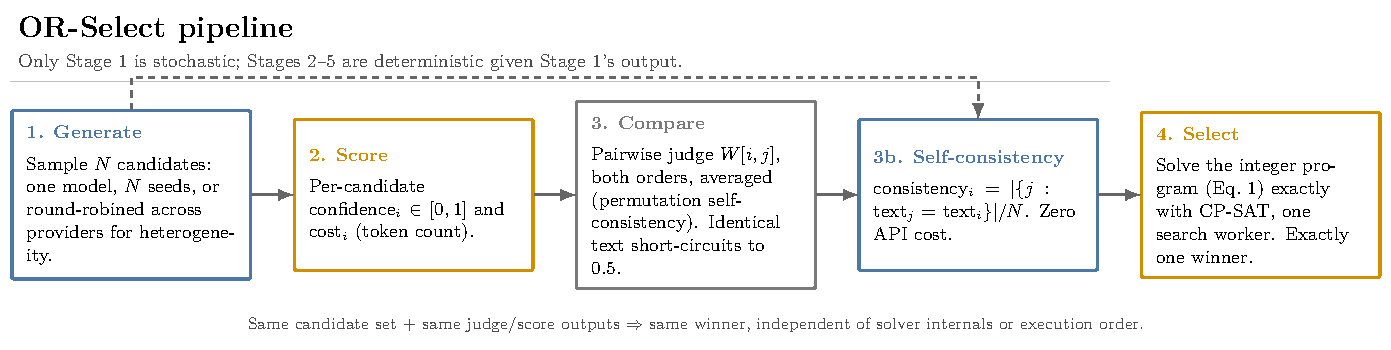
\includegraphics[width=\textwidth]{Figure_1_Pipeline.pdf}
\caption{OR-Select. Generation and judge calls may be stochastic; aggregation
and selection use their stored outputs. Self-consistency requires no API calls.}
\label{fig:pipeline}
\end{figure}

Sample $N$ candidates from one model or a round-robin model pool.
An invalid slot (for example, no extractable answer letter) is retried up
to three times with varied seeds; persistent failures are reported as
ungraded. Confidence $C_i\in[0,1]$ comes from a judge call, cost $c_i$ is
word count, and consistency $K_i=|\{j:\text{text}_j=\text{text}_i\}|/N$
counts exact full-text matches, unlike final-answer voting.

For each unordered pair, average the judge's forward score and the
complement of its reverse score to obtain $W[i,j]\in[0,1]$; set
$W[j,i]=1-W[i,j]$. This symmetrization mitigates order effects but does
not guarantee unbiased judging. Identical texts after trimming skip the
judge and receive $0.5$. At most $N(N-1)$ comparison calls are needed.
The quality aggregate is $Q_i=(N-1)^{-1}\sum_{j\ne i}W[i,j]$.

The two agreement signals serve different purposes. $Q_i$ measures how
strongly the judge prefers candidate $i$ to its competitors; $K_i$ measures
literal repetition of its complete response. Two derivations that end in
the same number can therefore contribute two votes to the self-consistency
baseline while each has $K_i=1/N$ in the composite objective. Confidence
is a separate pointwise judge assessment, not an observed correctness
frequency. Keeping these quantities separate makes it possible to remove
or reweight one without changing the saved comparisons.

\subsection{Formal Model}
\label{sec:formal-model}

Let $x_i$ indicate selection and $v_i$ denote validity. The selector solves

\begin{equation}
\max \sum_i x_i\left(w_1Q_i+w_2C_i+w_4K_i-w_3c_i\right)
\label{eq:selection-obj}
\end{equation}
\begin{align}
\text{s.t.}\quad & \sum_i x_i=1,\qquad x_i\in\{0,1\}, \\
& x_i\le v_i\quad\text{if some candidate is valid}, \\
& x_i=0\quad\text{if }Q_i<\text{min\_quality}\quad\text{(optional)}.
\end{align}

The default $(w_1,w_2,w_4,w_3)=(1,0.2,0.3,0.01)$ was fixed before
ground-truth runs, without tuning. A hundred-word difference therefore
costs one full quality unit. Without additional constraints, this
one-hot program is simply an argmax; integer programming provides a common
implementation for the eligibility constraints. CP-SAT \citep{perron2023ortools}
maximizes scores rounded after multiplication by $10^4$, using one worker.
Reproducibility is conditional on the stored inputs and solver environment;
this does not establish a canonical optimum across solver versions.

All terms are linear once the candidates have been scored. The validity
constraint excludes invalid candidates if at least one valid candidate
exists; an optional minimum-quality threshold excludes candidates below
that threshold. Thus feasibility restrictions and preference weights have
different roles. A low-cost response is not permitted to bypass an active
validity restriction, while an eligible response can win through a
combination of quality, confidence, consistency and cost. Reporting the
component scales is consequently important even when the final
optimization is computationally elementary.

Rows storing confidence and $W$ permit offline weight changes. The default
replay reproduces \AblationFidelityK/\AblationFidelityN{} extracted final
answers; this comparison is at the final-answer level. A worked example is
in the Appendix (Table~\ref{tab:worked-example}).

\subsection{Exact Kemeny--Young Baseline}
\label{sec:kemeny-exact}

For the ranking reference, let $y_{ij}=1$ mean that $i$ ranks above $j$.
The Kemeny--Young program maximizes agreement with the same matrix:

\begin{equation}
\max \sum_{i \neq j} W[i,j]\, y_{ij}
\label{eq:kemeny-obj}
\end{equation}
\begin{align}
\text{s.t.} \quad & y_{ij} + y_{ji} = 1 \quad \forall\, i \neq j \label{eq:kemeny-antisym}\\
& y_{ij} + y_{jk} + y_{ki} \leq 2 \quad \forall \text{ distinct } i,j,k \label{eq:kemeny-transitivity}\\
& y_{ij} \in \{0,1\}
\end{align}

Antisymmetry and the absence of 3-cycles enforce a linear order.
The implementation uses $\binom{N}{2}$ binary variables, $O(N^3)$
constraints and coefficients $\operatorname{round}(10^4(W[i,j]-W[j,i]))$.
A 200{,}000-conflict budget replaces a wall-clock limit; a non-optimality
flag distinguishes feasible from proven-optimal solutions. All
\KYTopOneN{} stored reference solutions at $N\le6$ are flagged optimal
for this integerized objective, not necessarily for unrounded weights.

The reference removes the composite selector's confidence, consistency and
cost terms and uses all pairwise relations simultaneously. With cyclic
preferences, its top-ranked candidate need not have the largest weighted
win total. This permits an empirical distinction between losing
information through aggregation and receiving unhelpful information from
the judge. We compare returned answers, rather than treating a difference
between rankings as an accuracy error. When two different candidates give
the same extracted answer, they count as the same answer-level decision.

\subsection{Approximation Guarantee}
\label{sec:approx-guarantee}

\begin{proposition}[Weighted-win ranking]
\label{prop:copeland-approx}
Assume nonnegative pair weights with $W[i,j]+W[j,i]=1$.
Ranking by decreasing $Q_i$ approximates minimum weighted disagreement
within a factor of 5. This factor is tight.
\end{proposition}

The constructed matrix satisfies these conditions. This guarantee, from
\citet{coppersmith2006ordering},
covers the \emph{full quality-only ranking}, not top-1 correctness, agreement
with the Kemeny winner, or the composite objective~\eqref{eq:selection-obj}.

\section{When can a judge beat voting? Pairwise-accuracy thresholds}
\label{sec:theory}

\paragraph{Model} Three candidates are independently correct with probability
$p$, all correct candidates share the same final answer, and wrong answers
are pairwise distinct. Plurality voting breaks answer ties uniformly.
Conditional on the correctness labels, the judge's three \emph{binary}
comparisons are independent: a mixed pair favors the correct candidate
with probability $q$, and a same-class pair is a fair coin. Copeland
selects the candidate with most wins, with an independent uniform tie-break.
This quality-only model differs from the empirical selector's averaged
soft scores and composite objective.

\begin{theorem}[Pairwise-accuracy threshold]
\label{thm:threshold}
Under the model above, the accuracy of the Copeland selector minus the accuracy of plurality
voting is
\[
\Delta(p,q)\;=\;p(1-p)\Bigl[(1-p)(2q-1)(q+1)\;-\;p\,(3-2q)(1-q)\Bigr].
\]
Hence, for $p\in(0,1)$ and $q<1$, the judge-based selector is strictly more accurate than voting
if and only if $\frac{p}{1-p}<\frac{(2q-1)(q+1)}{(3-2q)(1-q)}$; at $q=1$ it is always more accurate. In particular, (i) a judge at
chance ($q=\tfrac12$) selects with accuracy exactly $p$ and loses to voting by
$p^{2}(1-p)$; (ii) the unique break-even accuracy $q^{*}(p)$ increases strictly from $\tfrac12$
(as $p\to0$) to $1$ (as $p\to1$).
\end{theorem}

\begin{proof}
Conditional on exactly $k$ correct candidates, write $a_k$ for Copeland's
correct-selection probability. Then $a_0=0$, $a_3=1$.
With one correct candidate, winning both mixed comparisons succeeds;
winning exactly one succeeds only through a three-way tie, giving
$a_1=q^2+\tfrac13q(1-q)$. With two correct candidates, winning both
mixed comparisons succeeds; a split gives a correct selection with
probability $\tfrac12+\tfrac12\cdot\tfrac23=\tfrac56$, hence
$a_2=q^2+\tfrac53q(1-q)$. Plurality's conditional probabilities are
$(0,\tfrac13,1,1)$. Weighting by $\mathrm{Bin}(3,p)$ gives
\[
\Delta=3p(1-p)^2(a_1-\tfrac13)+3p^2(1-p)(a_2-1),
\]
which simplifies to the stated expression. At $q=\tfrac12$ it equals
$-p^2(1-p)$. On $(\tfrac12,1)$ the ratio in the theorem increases
continuously from zero to infinity: its numerator increases and its
positive denominator decreases. Equating it to $p/(1-p)$ establishes
uniqueness, monotonicity and the endpoint limits of $q^*$.
\end{proof}

At $p=0.8$, $q^*=0.803515\ldots$ (Table~\ref{tab:threshold}).
The formula gives both the sign and size of the gain under the model;
\texttt{scripts/judge\_threshold\_theory.py} checks it by exact enumeration.

An explicit expression for the break-even point is
\begin{equation}
q^*(p)=\frac{2(1+2p)}{1+4p+\sqrt{9+8p-16p^2}}.
\label{eq:threshold-root}
\end{equation}
It follows by setting $\Delta=0$ and rationalizing the relevant root of
$2(1-2p)q^2+(1+4p)q-(1+2p)=0$; the expression also covers $p=1/2$.
For $p=0.8$, plurality accuracy is $0.928$. A judge with $q=0.8$ yields
$0.92672$, just below voting, while $q=0.9$ yields $0.96128$, a gain of
$3.328$ percentage points. At $q=1$, the selector finds a correct candidate
whenever one exists, reaching $0.992$. Thus the threshold is not a claim
that judging cannot help: it identifies the reliability at which its
benefit overtakes the information already supplied by answer repetition.

\begin{table}[htbp]
\centering
\caption{Break-even binary judge accuracy $q^{*}$ at which the Copeland selector
ties plurality voting, as a function of the per-candidate accuracy $p$
(Theorem~\ref{thm:threshold}, $N=3$).}
\label{tab:threshold}
\small
\begin{tabular}{rr}
\toprule
$p$ & $q^{*}(p)$ \\
\midrule
\ThresholdRows
\bottomrule
\end{tabular}
\end{table}

\paragraph{Extensions and limits}
The Appendix (Section~\ref{sec:s-threshold}) enumerates
$N\le7$ and models wrong-answer collisions: each wrong candidate takes a
shared attractor with probability $\rho$, otherwise a distinct answer.
At $p=0.8,\rho=0$, the computed threshold rises from $0.804$ for $N=3$
to $0.945$ for $N=7$; at $\rho=0.5$ it is approximately $0.82$ for
$N=4,\ldots,7$. A monotone-coupling result bounds a pair-dependent
judge using its \emph{minimum and maximum} mixed-pair accuracies, not their
average (Corollary~\ref{cor:pairdep}). The appendix also gives a
large-$N$ threshold lower bound and consistency regimes. Neither candidate
independence nor uniform judge accuracy follows from a high aggregate
benchmark score, and asymptotic voting consistency does not exclude
finite-pool improvements by a stronger judge.

The finite-pool computation conditions on the number $k$ of correct
candidates. Let $a_{N,k}(q)$ denote the probability that a uniformly
tie-broken Copeland winner is correct. Enumerating all binary tournament
outcomes gives
\begin{equation}
A_J(N,p,q)=\sum_{k=0}^{N}\binom Nk p^k(1-p)^{N-k}a_{N,k}(q).
\label{eq:judge-general}
\end{equation}
With distinct wrong answers, plurality succeeds whenever $k\ge2$ and
with probability $1/N$ when $k=1$, so
\begin{equation}
A_V(N,p)=1-(1-p)^N-(N-1)p(1-p)^{N-1}.
\label{eq:vote-general}
\end{equation}
The computed break-even point equates these two accuracies. This is
exhaustive enumeration of the finite comparison model, not an estimate
from the benchmark observations; numerical root finding locates the
crossing to the reported precision. The appendix compares it with an
independent Monte Carlo calculation.

Table~\ref{tab:threshold-n} illustrates the effect of wrong-answer
collisions. Shared wrong answers strengthen the competing wrong vote,
whereas with distinct wrong answers two correct candidates suffice for
plurality to succeed. The collision model changes the voting calculation;
its binary judge still uses the stipulated mixed-pair accuracy. Its
parameter $\rho$ describes a common wrong answer, not arbitrary dependence
between candidate correctness events.

\begin{table}[htbp]
\centering
\caption{Finite-pool break-even binary accuracy $q^*(p,N,\rho)$, computed
by exhaustive tournament enumeration. A wrong candidate takes a shared
wrong answer with probability $\rho$, otherwise a distinct wrong answer.}
\label{tab:threshold-n}
\small
\begin{tabular}{rrrrr}
\toprule
 & \multicolumn{2}{c}{$\rho=0$} & \multicolumn{2}{c}{$\rho=0.5$} \\
\cmidrule(lr){2-3}\cmidrule(lr){4-5}
$N$ & $p=0.5$ & $p=0.8$ & $p=0.5$ & $p=0.8$ \\
\midrule
\ThresholdNRows
\ThresholdNSevenRow
\bottomrule
\end{tabular}
\end{table}

The pair-dependent extension uses a coupling rather than substituting an
average accuracy. Hold the correctness labels and comparison random
numbers fixed, and increase one mixed-pair accuracy. The only possible
change gives a correct candidate one additional win and a wrong candidate
one fewer win; the correct fraction of the top-score set cannot decrease.
Applying this change successively bounds selection accuracy between the
uniform-$q_{\min}$ and uniform-$q_{\max}$ cases. This provides a conservative
comparison when such bounds are available, without requiring every mixed
pair to have exactly the same reliability.

\subsection{Problems of differing difficulty}
\label{sec:mixture}

Theorem~\ref{thm:threshold} treats $p$ as common to all problems. In a
benchmark, difficulty varies: many problems are solved by every candidate or
by none, and only intermediate problems separate the rules. Let $p$ be drawn
per problem from a distribution $F$, with candidates and comparisons following
the model given $p$. Write $A(q)=(2q-1)(q+1)$ and $B(q)=(3-2q)(1-q)$, so that the
single-$p$ gap of Theorem~\ref{thm:threshold} is
$A(q)\,p(1-p)^2-B(q)\,p^2(1-p)$.

\begin{theorem}[Effective-odds threshold]
\label{thm:mixture}
Let $m_1=\mathbb{E}_F[p(1-p)^2]>0$ and $m_2=\mathbb{E}_F[p^2(1-p)]$. The accuracy of
Copeland minus that of plurality is $\Delta_F(q)=A(q)\,m_1-B(q)\,m_2$. It is positive
if and only if $A(q)/B(q)>r_F:=m_2/m_1$, so the break-even accuracy $q^*_F\in(\tfrac12,1]$
is the unique root of $A/B=r_F$ and increases with $r_F$.
\end{theorem}

The pooled threshold of Theorem~\ref{thm:threshold} is the special case
$F=\delta_{\bar p}$, where $r_F=\bar p/(1-\bar p)$. Dispersion changes $r_F$, so two
benchmarks with the same mean accuracy can have different break-even
judges; Table~\ref{tab:mixture} gives Beta examples. A problem set needs no
parametric $F$: if problem $i$ has $k_i$ of 3 candidates correct, the
conditional accuracy of Copeland is $a_{k_i}(q)$ (closed forms in the proof of
Theorem~\ref{thm:threshold}) and that of plurality is $0,\tfrac13,1,1$ for $k_i=0,\dots,3$.
Averaging over the observed $k_i$ gives a prediction that uses the
problems' own difficulty (Section~\ref{sec:mixture-results}).

\begin{table}[htbp]
\centering
\caption{Break-even binary accuracy $q^*_F$ when $p\sim\mathrm{Beta}$ with mean $\bar p$
and concentration $\kappa$ (smaller $\kappa$ means more dispersed difficulty);
the last column is the single-$p$ threshold at $\bar p$.}
\label{tab:mixture}
\small
\begin{tabular}{rrrrrr}
\toprule
$\bar p$ & $\kappa=1$ & $\kappa=2$ & $\kappa=5$ & $\kappa=20$ & $p\equiv\bar p$ \\
\midrule
\MixtureThresholdRows
\bottomrule
\end{tabular}
\end{table}

\subsection{Vote first, judge only on ties}
\label{sec:hybrid}

The model says more than a threshold. Because correct candidates share an
answer and wrong answers are distinct, any repeated answer is certainly
correct. A judge can only help when all $N$ answers differ. Rule~H returns a
most-voted answer and, if several answers tie, runs binary Copeland on the
comparisons among the tied candidates only.

\begin{theorem}[Vote-first fusion is optimal]
\label{thm:hybrid}
Under the model, for any $N\ge 2$ and $q\ge\tfrac12$, Rule~H attains the maximum
accuracy among all rules that observe the answer partition and the
comparison outcomes, namely
$P(k\ge2)+N\,p(1-p)^{N-1}\,a^{(N)}(q)$, where $a^{(N)}(q)\ge 1/N$ is the probability
that Copeland selects the lone correct candidate among $N$ distinct answers. Hence
Rule~H is at least as accurate as plurality and as Copeland for every $p$
and $q\ge\tfrac12$: it has no break-even threshold.
\end{theorem}

The proof (Appendix) is a Bayes argument: when all answers differ, the
posterior of a candidate being the only correct one is proportional to
$q^{w}(1-q)^{N-1-w}$, increasing in its number of wins $w$. Exhaustive
enumeration for $N\le4$ in exact rational arithmetic and for $N=5,6$ in floating
point confirms optimality and dominance. For example, at $N=6$, $p=0.3$ and
$q=0.8$ the accuracies of plurality, Copeland and Rule~H are $63.0\%$, $70.7\%$
and $77.1\%$ (Table~\ref{tab:hybrid-theory}). The result is a design principle
for fusion: spend judge calls only where votes are uninformative. It is proved
only for distinct wrong answers; when wrong answers collide, a wrong repeated
answer can outvote a lone correct one, Rule~H inherits that failure, and a
Copeland-based rule can recover it (Table~\ref{tab:threshold-n}).

\begin{table}[htbp]
\centering
\caption{Model accuracy (\%) of plurality, Copeland and Rule~H (exact enumeration).}
\label{tab:hybrid-theory}
\small
\begin{tabular}{rrrrrr}
\toprule
$N$ & $p$ & $q$ & Plurality & Copeland & Rule~H \\
\midrule
\HybridTheoryRows
\bottomrule
\end{tabular}
\end{table}

\section{Experimental Protocol}
\label{sec:experiments}

\subsection{Setup}
\label{sec:setup}

The fixed judge is NVIDIA Nemotron-3.5-Lightning on OpenRouter
(\texttt{\seqsplit{nvidia/nemotron-3.5-lightning:free}}), with reasoning
disabled and a 256-token cap; truncated judge replies raise errors.
Homogeneous pools contain $N=3$ Nemotron draws with distinct seeds.
Heterogeneous pools contain $N=6$ draws, initially two each from Nemotron,
Poolside Laguna-S~2.1 and Cohere North-Mini-Code. After Laguna's withdrawal,
Xing4.0-29B filled its slots (\SelectionXingchenCands{} candidates);
one early GPQA problem retains two LFM-2.5 candidates. This pool drift is
reported, not treated as a fixed three-model experiment.

Generation uses a 32{,}768-token cap and varied-seed retries. A flagged
second pass retries ungraded problems at 65{,}536 tokens, subject to model
ceilings. Tables~\ref{tab:coverage}--\ref{tab:extended} report coverage,
pool composition and accuracy with and without these rescued problems.

The main references are self-consistency (plurality over extracted final
answers, candidate-order ties), the \emph{first sampled candidate} (not
temperature-zero greedy decoding), and the Kemeny--Young top-ranked answer
on the same matrix. Further offline selectors are listed in
Section~\ref{sec:baselines}. Trained verifiers and universal
self-consistency were not evaluated.

\paragraph{Judge calibration}
\label{sec:rewardbench-setup}

RewardBench \citep{rewardbench2025} uses the same forward/backward judging
path: its combined score must favor the human-preferred answer. The
pre-registered sample takes the first seven rows of each of 23 subsets
($n=161$), not a random sample. Overall accuracy averages category means;
the appendix also reports a micro-average and its Wilson interval.

\subsection{Evaluation tracks}
\label{sec:tracks}

Six homogeneous tracks comprise \TotalProblems{} distinct problems:
B, 40 GSM8K test items \citep{cobbe2021gsm8k}; C, all 134 Level-5 items
of MATH-500 \citep{hendrycks2021math,lightman2023letsverify}; D, 30 AIME
2026 problems \citep{matharena2025aime}; E, all 198 GPQA Diamond items
\citep{rein2024gpqa}; F, 30 AIME 2025 problems; and G, 100 MMLU-Pro test
items \citep{wang2024mmlupro}. B--E are repeated with heterogeneous pools
on the same 402 problems, not additional independent benchmark items.
MMLU-Pro samples five consecutive items at each of 20 evenly spaced
offsets, covering 12 of 14 subjects. AIME 2025 may be contaminated because
it predates the generator; it is a robustness check.

GSM8K uses the last number; MATH uses normalized exact match of the last
\texttt{\textbackslash boxed\{\}} answer; AIME uses the extracted integer;
GPQA and MMLU-Pro use exact letters. String-based mathematics grading can
reject equivalent expressions. The three-query open-ended pilot has no
ground truth and is supplementary only (Section~\ref{sec:pilot}).

\subsection{Metrics}
\label{sec:metrics}

We report graded/benchmark-total coverage and exact two-sided McNemar tests
on paired discordant problems \citep{fagerland2013mcnemar}; pooled tests sum
discordances within each generation condition. The test form was
pre-registered, but the added tracks and six-track homogeneous pooling were
not; pooled findings, per-track comparisons and ablations are exploratory,
without multiplicity correction. A non-significant test is not equivalence.

The \emph{floor} is mean candidate accuracy (uniform random selection),
not a performance lower bound; the \emph{oracle} is the proportion with
at least one correct candidate. Recovery is
$(\mathrm{acc}-\mathrm{floor})/(\mathrm{oracle}-\mathrm{floor})$
\citep[cf.][]{landesberg2026bestofn}, reported only when headroom is positive.
Negative recovery means worse than a random pick.

\section{Results}
\label{sec:results}

\subsection{Judge validation: RewardBench}
\label{sec:rewardbench-results}

The fixed judge scores \RBOverallAcc\% overall, reaching
\RBReasoningAcc\% on reasoning pairs (\RBReasoningCorrect/\RBReasoningRows).
Rotating judges yields \RBXOverallAcc\%; this exploratory result informed
retaining one fixed judge. Table~\ref{tab:rewardbench} separates the
categories. This calibration evaluates agreement with human-preferred
responses; it is not the binary correct-versus-wrong parameter of the
threshold model. Micro-averaging, length diagnostics and configuration
history appear in Section~\ref{sec:judge-diagnostics} of the Online
Supplement.

\begin{table}[htbp]
\centering
\caption{Fixed-judge RewardBench accuracy by category ($n=\RBN$).
The overall score is the mean of category accuracies.}
\label{tab:rewardbench}
\begin{tabularx}{\textwidth}{Xrr}
\toprule
Category & Rows & Accuracy \\
\midrule
Reasoning (math-prm and six \texttt{hep-*} code subsets) & \RBReasoningRows & \RBReasoningAcc\% \\
Chat & \RBChatRows & \RBChatAcc\% \\
Chat Hard (adversarial LLMBar subsets) & \RBChatHardRows & \RBChatHardAcc\% \\
Safety & \RBSafetyRows & \RBSafetyAcc\% \\
\bottomrule
\end{tabularx}
\end{table}

\subsection{Accuracy against the baselines}
\label{sec:accuracy-results}

Tables~\ref{tab:tracks}--\ref{tab:paired} report accuracy and paired
discordances. Across \HomogPooledN{} homogeneous problems, OR-Select
alone is correct on \HomogPooledB{} and self-consistency alone on
\HomogPooledC{} (\HomogPooledP): a difference of $-0.56$ percentage
points, without a detected advantage. Across \HeteroPooledN{} heterogeneous
problems the counts are \HeteroPooledB{} versus \HeteroPooledC{}
(\HeteroPooledP), a $-5.47$-point difference. This loss comes from GSM8K,
MATH and AIME 2026. Heterogeneous GPQA instead favors OR-Select numerically
(10 versus \SCwinsGPQAx{} discordances, $p=0.454$), so the pooled result
is not uniform across tasks.

\begin{table}[htbp]
\centering
\caption{Accuracy (\%) on graded problems, by track and selector. `--': no
Kemeny--Young comparator (GSM8K). Bold: best of the three practical
selectors when they differ. Primed rows: heterogeneous generation.}
\label{tab:tracks}
\small\setlength{\tabcolsep}{4pt}
\resizebox{\textwidth}{!}{%
\begin{tabular}{lrrrrr}
\toprule
Track & Graded/Total & First sample & Self-cons.\ & OR-Select & Kemeny--Young \\
\midrule
\TracksTableRows
\bottomrule
\end{tabular}}
\end{table}

\begin{table}[htbp]
\centering
\caption{Paired comparison of OR-Select with each reference selector. Cells
give (problems where OR-Select is right and the reference wrong)/(the
reverse) and the exact two-sided McNemar $p$-value.}
\label{tab:paired}
\small\setlength{\tabcolsep}{3pt}
\resizebox{\textwidth}{!}{%
\begin{tabular}{lrrrrrr}
\toprule
Track & vs.\ SC & $p$ & vs.\ first sample & $p$ & vs.\ Kemeny--Young & $p$ \\
\midrule
\PairedTableRows
\bottomrule
\end{tabular}}
\end{table}

\subsection{Headroom and recovery}
\label{sec:recovery}

Table~\ref{tab:recovery} distinguishes saturation from failed selection.
Homogeneous GSM8K has no headroom; homogeneous GPQA has roughly ten
percentage points, of which both selectors recover 16\%.
OR-Select falls below the random-pick floor on heterogeneous MATH and
AIME 2026, whereas its numerical recovery advantage on heterogeneous GPQA
is not statistically significant (Table~\ref{tab:paired}).

\begin{table}[htbp]
\centering
\caption{Headroom and recovery on graded problems. Floor: mean candidate
accuracy. Oracle: some candidate correct. Recovery (\%):
$(\text{acc}-\text{floor})/(\text{oracle}-\text{floor})$; negative means
below a random pick.}
\label{tab:recovery}
\small\setlength{\tabcolsep}{4pt}
\resizebox{\textwidth}{!}{%
\begin{tabular}{lrrrrrrr}
\toprule
Track & Graded & Floor & SC & OR & Oracle & Rec.\ SC & Rec.\ OR \\
\midrule
\RecoveryTableRows
\bottomrule
\end{tabular}}
\end{table}

\subsection{Objective and selection diagnostics}
\label{sec:selection-bias}
\label{sec:cost-diagnosis}
\label{sec:ablations}

On replayable problems, the within-pool cost-term spread has median
\CostSpreadMed{}, versus \QualitySpreadMed{} for quality, and exceeds
the quality spread in \CostDominatesK/\CostDominatesN{} cases. This
exposes a scale mismatch, not a proof that cost determines every winner:
confidence, consistency, eligibility and score gaps also matter.

Table~\ref{tab:ablation} compares the default, no-cost, quality-only and
plurality-plus-quality variants on identical replayable subsets. In
heterogeneous pools, removing cost yields \AblHetNoCostAcc\% accuracy and
quality-only selection \AblHetQOnlyAcc\%, against voting's
\AblHetSCAcc\% ($n=\AblHetN$; exact $p$ \AblHetNoCostP{} and
\AblHetQOnlyP{}, respectively). Thus the cost term is not the only
limitation. These post-hoc results do not prove that the judge contains
no useful correctness information.

OR-Select picks Cohere candidates in \PickShareCohere\% of heterogeneous
problems, although their overall accuracy (\CandAccCohere\%) is similar to
Nemotron's (\CandAccNemotron\%). This is a property of the \emph{composite
selector}, not an isolated judge preference; length and other terms are
confounded (Table~\ref{tab:selection}).

\begin{table}[htbp]
\centering
\caption{Offline replay of the selection step on stored judge outputs
(accuracy \%, problems whose judge outputs were stored). SC: stored
self-consistency result on the same problems.}
\label{tab:ablation}
\small\setlength{\tabcolsep}{4pt}
\resizebox{\textwidth}{!}{%
\begin{tabular}{lrrrrrr}
\toprule
Track & Replayable & SC & Default & No cost & Quality only & SC+quality \\
\midrule
\AblationTableRows
\bottomrule
\end{tabular}}
\end{table}

\paragraph{Additional selectors}
\label{sec:baselines}

Shortest/longest, token-Jaccard minimum-Bayes-risk, pointwise confidence,
confidence-weighted voting, a knockout tournament and Bradley--Terry
selection establish no significant improvement over plurality in the
exploratory comparisons (Table~\ref{tab:baselines}). Minimum-Bayes-risk
is numerically ahead in some pooled comparisons, without a significant advantage.

\paragraph{Soft-score diagnostics}
\label{sec:threshold-results}

The mean stored weight assigned to the correct candidate on mixed pairs
is $0.49$--$0.56$ on tracks with at least 70 such pairs. These are
\emph{soft-score means}, not frequencies of correct binary decisions.
They cannot be substituted for $q$ in Theorem~\ref{thm:threshold}; neither
can an average establish the pairwise bounds of Corollary~\ref{cor:pairdep}.
Table~\ref{tab:threshold-emp-gen} retains these descriptive measurements
and model sensitivity calculations, with their sampling limitations.

\subsection{Difficulty-aware prediction}
\label{sec:mixture-results}

On the homogeneous problems with stored judge outputs and at least ten mixed
pairs ($n=\MixPooledN$, AIME 2025 and MMLU-Pro; GSM8K has no stored judgments and
MATH Level 5 and AIME 2026 have too few mixed pairs), the binary mixed-pair
accuracy is $\MixPooledQ\%$. Using each problem's own number of correct
candidates $k_i$ and this $q$, the model predicts binary-Copeland accuracy
$\MixPooledPredCop\%$; the observed value is $\MixPooledObsCop\%$ (bootstrap
interval for observed minus predicted, re-estimating $q$ in each resample:
$[\MixPooledErrLo,\MixPooledErrHi]$ points). A pooled-$p$ prediction under the
single-$p$ binomial model gives $\MixPooledNaiveCop\%$. The two agree on Copeland but not on plurality: observed plurality
accuracy is $\MixPooledObsVote\%$, the own-$k$ model gives $\MixPooledPredVote\%$ and the pooled-$p$ model
$\MixPooledNaiveVote\%$, because the binomial model puts too little mass on problems solved by
none or one candidate. The resulting gap prediction (Copeland minus plurality, in points)
is $\MixPooledGapPred$ with own $k_i$ against $\MixPooledGapNaive$ pooled, for an observed
$\MixPooledGapObs$ (Table~\ref{tab:mixture-emp}). The sample is small and $q$ is estimated on the
same rows, so this is a plug-in consistency check, not out-of-sample validation;
MMLU-Pro's binary $q$ lies below one half on 28 mixed pairs.

\begin{table}[htbp]
\centering
\caption{Observed and predicted binary-Copeland accuracy (\%) and the Copeland-minus-plurality
gap (points). Pred.\ ($k_i$) uses each problem's own number of correct candidates;
Pred.\ ($\bar p$) uses the single-$p$ binomial model at the pooled accuracy.}
\label{tab:mixture-emp}
\scriptsize
\setlength{\tabcolsep}{3pt}
\begin{tabular}{lrrrrrrrrr}
\toprule
 & & & & \multicolumn{3}{c}{Copeland accuracy} & \multicolumn{3}{c}{Gap} \\
\cmidrule(lr){5-7}\cmidrule(lr){8-10}
Track & $n$ & $\hat p$ & $\hat q$ & Obs. & $k_i$ & $\bar p$ & Obs. & $k_i$ & $\bar p$ \\
\midrule
\MixtureEmpiricalRows
\bottomrule
\end{tabular}
\end{table}

\subsection{Vote-first fusion on stored runs}
\label{sec:hybrid-results}

Rule~H is computed offline on every graded problem with stored judge outputs
($\HybHomN$ homogeneous and $\HybHetN$ heterogeneous problems; Table~\ref{tab:hybrid-audit}).
Exact vote ties are rare: $\HybHomTies$ and $\HybHetTies$ problems, of which only
$\HybHomOpp$ and $\HybHetOpp$ contain a correct candidate. Rule~H therefore tracks voting:
$\HybHetHyb\%$ against $\HybHetSC\%$ in heterogeneous pools ($\HybHetBSC$ versus $\HybHetCSC$ discordant
problems, $p=\HybHetPSC$) and $\HybHomHyb\%$ against $\HybHomSC\%$ in homogeneous pools
($\HybHomBSC$ versus $\HybHomCSC$, $p=\HybHomPSC$). Against Copeland alone it is better in heterogeneous
pools ($\HybHetBCop$ versus $\HybHetCCop$ discordant problems, $p=\HybHetPCop$) and indistinguishable
in homogeneous pools ($\HybHomBCop$ versus $\HybHomCCop$). Using the judge only on ties thus removes
the heterogeneous-pool penalty of judging everywhere, but with the tested judge it adds no
detectable accuracy over voting, as expected when its binary accuracy is near chance. The stored
voting baseline breaks ties by candidate order, and the judged subset is not a random sample;
GPQA Diamond is not part of this audit because its stored outputs are not in the public archive.

\begin{table}[htbp]
\centering
\caption{Rule~H on stored runs. Ties: problems where several answers tie for most votes; Opp.:
ties containing a correct candidate. Accuracy in \%. Discordant counts are problems won by
Rule~H and lost by the comparator, with the exact two-sided McNemar $p$ in parentheses.}
\label{tab:hybrid-audit}
\scriptsize
\setlength{\tabcolsep}{3pt}
\begin{tabular}{lrrrrrrr}
\toprule
Track & $n$ & Ties/Opp. & Vote & Copeland & Rule H & H vs.\ vote & H vs.\ Copeland \\
\midrule
\HybridAuditRows
\bottomrule
\end{tabular}
\end{table}

\subsection{Ranking reference and coverage}
\label{sec:kemeny-results}

OR-Select and the integerized Kemeny--Young reference return different
final answers on \KYTopOneDiffers/\KYTopOneN{} problems. OR-Select alone
is correct on \KYORwins{} and Kemeny--Young alone on \KYKYwins{}
(Table~\ref{tab:paired}); the exact ranking reference shows no detected
accuracy advantage. Ranking optimality does not guarantee correctness.

\paragraph{Coverage}
\label{sec:coverage}

Every problem is ultimately graded (Table~\ref{tab:coverage}). Including
the higher-cap rescued problems lowers selector accuracy by 0.3--15 points
depending on track, without reversing the direction of the comparisons
(Table~\ref{tab:extended}). These results describe the retry-conditioned
generation protocol, not unrestricted independent draws.

\section{Discussion}

\paragraph{Interpretation}
The audit supports evaluating the entire decision rule on fixed candidate
pools: a ranking objective can fit judge preferences without improving
correctness, and an unnormalized cost term can overshadow a bounded quality
score. Stored outputs make these distinctions inspectable without new API
calls. The theory separately quantifies the trade-off for independent binary
comparisons. Connecting it to soft-score selection requires assumptions
about score distributions and dependence, not merely a mean score.

\paragraph{Scope}
\label{sec:future}

Only one free-tier fixed judge is evaluated in the main audit. Stronger
judges, trained verifiers and other selection architectures may perform
differently. Forward--reverse averaging addresses position bias; style bias,
reported to be larger in other judge benchmarks \citep{soumik2026judging},
is not controlled, and a debiasing comparison on this pool is left open. Small discordant counts limit precision; the replay subset is
not randomly sampled, and mixed-pair measurements are sparse on several
tracks. Candidate-order voting ties can favor particular generators in the
round-robin pool. The reported results describe the generation, extraction
and retry protocols of Section~\ref{sec:experiments}. The theory assumes
independent candidate correctness and
conditionally independent comparisons; the wrong-answer collision model
does not model general correlated errors.

\section{Conclusion}

An exact finite-$N$ calculation specifies when binary Copeland selection
beats plurality under a stylized model; with varying difficulty the
break-even accuracy is set by an effective-odds ratio rather than pooled
accuracy, and a vote-first rule that judges only on ties is optimal in the model
and has no break-even threshold. A separate six-benchmark audit
finds no detected homogeneous-pool advantage for the tested free-tier judge
and a pooled heterogeneous-pool loss; on stored runs, vote-first selection
removes that loss but, because exact ties are rare and the judge is near
chance, adds no detectable accuracy over voting. The exact Kemeny reference and
offline ablations distinguish ranking fit, objective design and answer
accuracy. Together, the finite-pool calculation and stored-output audit
separate the reliability needed by a specified selection rule from the
performance observed for a particular judge configuration.

\section*{Data and code availability}
Code, tables, pre-registration documents and run files are provided in an
anonymized archive with this submission; a public, permanently archived release
will be cited in the camera-ready version. The run archive excludes GPQA
records containing password-gated question text; access to that benchmark
follows its distribution conditions. The analysis scripts regenerate all tables
from stored runs and include the GPQA generation workflow.

\bibliographystyle{tmlr}
\bibliography{refs}

\appendix
\renewcommand{\thetable}{\Alph{section}.\arabic{table}}
\renewcommand{\thefigure}{\Alph{section}.\arabic{figure}}
\section{Extended threshold analysis}
\label{sec:s-threshold}

This section extends Section~\ref{sec:theory} beyond $N=3$. Unless stated
otherwise, candidates are independent and, conditional on their correctness
labels, comparisons are independent, same-class comparisons are fair, and
top-score ties are broken uniformly. The results concern binary comparisons,
not the empirical pipeline's averaged soft weights.

\begin{lemma}[Monotone coupling]
\label{lem:monotone}
For every $N$ and every $\rho$, the probability that the Copeland selector
returns a correct candidate is nondecreasing in each $q_{ij}$.
\end{lemma}

\begin{corollary}[Pair-dependent judges]
\label{cor:pairdep}
Let $q^{*}(p,N,\rho)$ be the smallest uniform $q$ at which the selector ties
voting. A judge with $q_{ij}\ge q^{*}$ for all mixed pairs is at least as accurate
as voting; one with $q_{ij}\le q^{*}$ for all mixed pairs is at most as accurate.
\end{corollary}

Table~\ref{tab:threshold-n} gives $q^{*}$ computed exactly for $N=3,\dots,7$
(the $N=3$, $\rho=0$ column reproduces Table~\ref{tab:threshold}). Two things stand
out. With distinct wrong answers the computed threshold rises over $N=3,\ldots,7$:
at $p=0.8$ it goes from $0.804$ to $0.945$. Proposition~\ref{prop:lower}
also gives a large-$N$ lower bound. With correlated wrong answers ($\rho=0.5$) voting is weaker
and the threshold is lower, about $0.82$ at $p=0.8$ for $N\ge4$. The
direction of the relaxation is therefore the one a reader would expect, but its
size is large enough that the realistic threshold is far from $\tfrac12$.
For parameters estimated from homogeneous GPQA Diamond, the model threshold
falls from $0.787$ to $0.714$ (Table~\ref{tab:threshold-emp-gen}).
The recorded soft-score mean is not an estimate of binary accuracy $q$.
We checked the exact enumeration against an independent Monte Carlo
simulation with common random numbers (Table~\ref{tab:threshold-valid}; all
four configurations agree within sampling error) and checked
Corollary~\ref{cor:pairdep} on random pair-dependent judges: in
\PairDepInside{} of \PairDepTrials{} random $N=5$ instances the accuracy gap lies
between the gaps at $q_{\min}$ and $q_{\max}$.

\begin{table}[htbp]
\centering
\caption{Exact accuracy gap (Copeland minus plurality, percentage points) against a
200{,}000-draw Monte Carlo estimate with its standard error.}
\label{tab:threshold-valid}
\small
\begin{tabular}{rrrrrr}
\toprule
$N$ & $p$ & $\rho$ & $q$ & Exact & Monte Carlo \\
\midrule
\ThresholdValidationRows
\bottomrule
\end{tabular}
\end{table}

\paragraph{Why the threshold keeps rising: a large-$N$ lower bound}
With distinct wrong answers plurality's error has a closed form. It is correct
whenever at least two candidates are correct, and when exactly one is correct all $N$ answers
differ and it is chosen with probability $1/N$, so
\begin{equation}
\mathrm{err}_{V}(N)=(1-p)^{N}+(N-1)\,p\,(1-p)^{N-1},
\label{eq:vote-err}
\end{equation}
which decays at rate $-\ln(1-p)$ per candidate. A pairwise-Copeland selector
that errs on the event ``a wrong candidate beats a sizeable block of correct ones''
decays more slowly unless $q$ is large. Write
$\mathrm{KL}(\eta\Vert p)=\eta\ln\frac{\eta}{p}+(1-\eta)\ln\frac{1-\eta}{1-p}$ and
\[
\Lambda(p,q)\;=\;\inf_{1-\frac{1}{2q}<\eta\le1}\Bigl[\mathrm{KL}(\eta\Vert p)+\eta\ln\tfrac{1}{1-q}\Bigr].
\]

\begin{proposition}[Large-$N$ lower bound]
\label{prop:lower}
Let wrong answers be distinct ($\rho=0$) and the judge uniform with $\tfrac12<q<1$. If
$\Lambda(p,q)<-\ln(1-p)$, there is $N_0$ such that for all $N\ge N_0$ the Copeland selector is strictly
less accurate than plurality. Consequently $\liminf_{N\to\infty}q^{*}(p,N)\ge q_{\Lambda}(p)$, where
$q_{\Lambda}(p)$ is the unique root of $\Lambda(p,q)=-\ln(1-p)$.
\end{proposition}

Table~\ref{tab:threshold-lambda} lists $q_{\Lambda}(p)$ next to the exact $N=6$ thresholds:
the exact values sit just below the limiting lower bound for $p\ge0.6$ and just above it at $p=0.5$,
as a sequence rising to (at least) $q_{\Lambda}$ would. We do not prove that the limit equals $q_{\Lambda}$; the
proposition is a lower bound, obtained by exhibiting one specific way in which Copeland errs.

\begin{table}[htbp]
\centering
\caption{Plurality's error decay rate $-\ln(1-p)$, the large-$N$ lower bound $q_{\Lambda}(p)$ on
$\liminf_N q^{*}(p,N)$ (Proposition~\ref{prop:lower}), and the exact $q^{*}(p,6)$ ($\rho=0$).}
\label{tab:threshold-lambda}
\small
\begin{tabular}{rrrr}
\toprule
$p$ & $-\ln(1-p)$ & $q_{\Lambda}(p)$ & $q^{*}(p,6)$ \\
\midrule
\ThresholdLambdaRows
\bottomrule
\end{tabular}
\end{table}

\paragraph{Structure of the wrong answers beyond a single attractor}
The attractor model with parameter $\rho$ is one way to correlate wrong answers. We also
drew each wrong answer uniformly from $D$ wrong values ($D=1$: all wrong answers coincide;
$D=3$: the three distractors of a four-option question; $D=\infty$: all distinct).
Table~\ref{tab:threshold-D} shows that the threshold is monotone in the structure: the fewer distinct wrong values, the
weaker plurality and the lower the threshold, down to $q^{*}=\tfrac12$ when all wrong answers coincide and the
pool is small ($N=4$, $p=0.5$). For the four-option GPQA questions ($D=3$) the threshold is $0.64$--$0.80$ at
$N=4,5$, illustrating sensitivity to wrong-answer structure rather than
validating the attractor model for GPQA.

\begin{table}[htbp]
\centering
\caption{Exact $q^{*}$ when each wrong answer is uniform over $D$ wrong values.}
\label{tab:threshold-D}
\small
\begin{tabular}{rrrrr}
\toprule
 & \multicolumn{2}{c}{$N=4$} & \multicolumn{2}{c}{$N=5$} \\
\cmidrule(lr){2-3}\cmidrule(lr){4-5}
$D$ & $p=0.5$ & $p=0.8$ & $p=0.5$ & $p=0.8$ \\
\midrule
\ThresholdDRows
\bottomrule
\end{tabular}
\end{table}

\paragraph{The cost term} The thresholds concern quality-only selection.
Table~\ref{tab:threshold-cost} illustrates adding independent random lengths
in one simulation. A dominant cost term selects the shortest candidate;
when lengths are independent of correctness and ties have probability zero,
that rule has accuracy $p$. This limiting argument does not prove monotone
accuracy degradation for every cost distribution or judge. Empirical lengths
are not independent of correctness, so Section~\ref{sec:cost-diagnosis}
evaluates their effect by replay.

\begin{table}[htbp]
\centering
\caption{Simulated accuracy (\%) of selection by Copeland score minus $\lambda\times$ an independent random
length, $N=3$, $p=0.8$ (plurality voting: 92.8\%; random pick: 80.0\%), 100{,}000 draws.}
\label{tab:threshold-cost}
\small
\begin{tabular}{lrr}
\toprule
$\lambda$ & $q=0.6$ & $q=0.9$ \\
\midrule
\ThresholdCostRows
\bottomrule
\end{tabular}
\end{table}

\paragraph{Large-$N$ consistency} When both selectors approach perfect
accuracy, their error rates can still differ. The following consistency
result complements, rather than replaces, the threshold comparison.

\begin{proposition}[Large-$N$ regimes]
\label{prop:regimes}
Let candidates be independent with correct-answer probability $p>0$, wrong answers taking finitely many values, and let $m$ be the largest probability of any single wrong answer. (i) Plurality voting
is correct with probability tending to $1$ if $p>m$ and to $0$ if $p<m$. (ii) If
$q_{ij}\ge q_{\min}>\tfrac12$ for all mixed pairs, the Copeland selector is
correct with probability at least $1-(1-p)^N-2N^{2}e^{-(q_{\min}-1/2)^{2}N/2}\to1$,
whatever $m$.
\end{proposition}

A better-than-chance judge can therefore rescue a pool when $p<m$, where
plurality fails asymptotically. When $p>m$, both may be consistent; this does
not determine their finite-$N$ difference. Aggregate accuracy across prompts
does not identify the regime of each prompt. The distinction parallels
reward-based selection analyses \citep{di2025bom}, without establishing a
universal explanation for the empirical results.


\section{Proofs for the extended threshold analysis}
\label{sec:s-proofs}

\label{app:proof2}

\emph{Lemma~\ref{lem:monotone}.} Fix a mixed pair $(c,w)$ with $c$ correct and $w$ wrong and
condition on all other comparison outcomes; the outcome of $(c,w)$ is a
Bernoulli($q_{cw}$) variable that is the only one depending on $q_{cw}$, so it
suffices to show that changing it from ``$w$ wins'' to ``$c$ wins'' cannot lower the
probability that the selected candidate is correct. The change raises $c$'s score by one and lowers $w$'s by one.
Let $T$ be the set of top scorers before and $T'$ after, and let the selected candidate be uniform on the top set, so the success
probability is the share of correct candidates in it. If $c\in T$, then $T'=\{c\}$, which is correct. If
$c\notin T$ and $w\notin T$, then $T'=T$ or $T'=T\cup\{c\}$; adding a correct candidate cannot lower a
share that is at most one. If $w\in T$ and $|T|>1$, then $T'$ removes $w$ and possibly adds $c$, which
cannot lower the share. If $w$ is the unique top scorer, the share before is $0$. In every case the share does not decrease.
Averaging over the other outcomes gives the claim, and Corollary~\ref{cor:pairdep} follows by comparing with the uniform judges at $q_{\min}$
and $q_{\max}$ (voting does not depend on the judge).

\emph{Proposition~\ref{prop:regimes}.} (i) The count of the correct answer is Binomial$(N,p)$ and that of each wrong answer is Binomial$(N,\cdot)$ with success probability at most $m$, the largest attaining $m$; by Hoeffding's inequality and a union bound over the finitely many answers, the correct answer is the unique plurality with probability tending to one if $p>m$, and is beaten by the most popular wrong answer with probability tending to one if $p<m$. (ii) Condition on the set of correct candidates, of size $k_c\ge1$ (probability $1-(1-p)^N$), and let
$k_w=N-k_c$. A correct candidate's score is a sum of $N-1$ independent comparisons with mean at least
$q_{\min}k_w+\tfrac12(k_c-1)$; a wrong candidate's has mean at most $(1-q_{\min})k_c+\tfrac12(k_w-1)$; the
difference is at least $(q_{\min}-\tfrac12)N$. By Hoeffding's inequality each score is within
$t=(q_{\min}-\tfrac12)N/2$ of its mean with probability at least
$1-2\exp(-2t^2/(N-1))\ge1-2\exp(-(q_{\min}-\tfrac12)^2N/2)$. A union bound over the $N$ candidates gives
the stated probability that every correct candidate outscores every wrong one, in which case the selected
candidate is correct. \qed

\emph{Equation~\eqref{eq:vote-err}.} With distinct wrong answers the plurality is the correct answer exactly when
at least two candidates are correct (its count then exceeds every wrong count, which is one); with one correct candidate
all $N$ answers are tied and the correct one is chosen with probability $1/N$; with none it cannot be chosen. Hence
$\mathrm{err}_V=(1-p)^N+Np(1-p)^{N-1}(1-1/N)$.

\emph{Proposition~\ref{prop:lower}.} Fix $q>\tfrac12$ and $\eta\in(1-\tfrac1{2q},1)$ and let $K=\lceil\eta N\rceil$. Consider the event $E$ that
exactly $K$ candidates are correct and a designated wrong candidate $w$ beats all of them (probability
$\binom NK p^K(1-p)^{N-K}(1-q)^K\ge \frac{1}{N+1}e^{-N\,\mathrm{KL}(K/N\Vert p)}(1-q)^K$). Conditionally on $E$, $w$'s score is $K+\mathrm{Bin}(N-K-1,\tfrac12)$,
with mean $(N+K-1)/2$; a correct candidate's score has mean at most $q(N-K-1)+(K-1)/2+0$ (it has already lost to $w$), and another wrong
candidate's has mean $(1-q)K+(N-K-1)/2$. The gaps are $N(\tfrac12-q(1-\eta))+O(1)$ and $qK$, linear in $N$ and positive because
$\eta>1-\tfrac1{2q}$. By Hoeffding's inequality and a union bound over the $N$ candidates, $w$ is the unique top scorer with conditional probability
$1-O(N e^{-cN})$, so the Copeland selector errs on $E$ with probability at least $\tfrac12$ for large $N$. Therefore
$\mathrm{err}_C\ge\frac{1}{2(N+1)}e^{-N[\mathrm{KL}(\eta\Vert p)+\eta\ln\frac1{1-q}+o(1)]}$. If $\Lambda(p,q)<-\ln(1-p)$ choose $\eta$
with bracket below $-\ln(1-p)$; since $\mathrm{err}_V\le N(1-p)^{N-1}$ by Equation~\eqref{eq:vote-err}, $\mathrm{err}_C>\mathrm{err}_V$ for all large $N$.
For the consequence: $\Lambda(p,q)$ is continuous and strictly increasing in $q$ (it equals an infimum of functions
increasing in $q$ over a set that shrinks with $q$), lies below $-\ln(1-p)$ for $q$ slightly above $\tfrac12$ (the derivative of $\mathrm{KL}(\eta\Vert p)$ is $-\infty$ at $\eta=0$) and
diverges as $q\uparrow1$ (it is at least $\tfrac12\ln\frac1{1-q}$), so $q_\Lambda(p)$ exists and is unique. For any $\epsilon>0$ the accuracy gap at $q_\Lambda-\epsilon$ is negative for large
$N$, and by Lemma~\ref{lem:monotone} it is nonincreasing as $q$ decreases, so it is negative for every $q\le q_\Lambda-\epsilon$. Hence
$q^{*}(p,N)>q_\Lambda-\epsilon$ for large $N$. \qed

\section{Proofs for the difficulty-mixture and vote-first results}
\label{sec:s-new-proofs}

\emph{Theorem~\ref{thm:mixture}.} By Theorem~\ref{thm:threshold} the accuracy gap for a fixed $p$ is
$\Delta(p,q)=p(1-p)\bigl[(1-p)(2q-1)(q+1)-p(3-2q)(1-q)\bigr]=A(q)\,p(1-p)^2-B(q)\,p^2(1-p)$.
Selection and comparison randomness are conditionally independent of $F$ given $p$, so the mixture gap is
$\mathbb{E}_F\Delta(p,q)=A(q)\,m_1-B(q)\,m_2$ by linearity. On $(\tfrac12,1]$, $A$ is strictly increasing
from $A(\tfrac12)=0$ to $A(1)=2$, and $B$ is strictly decreasing from $B(\tfrac12)=1$ to $B(1)=0$, so
$A/B$ increases strictly from $0$ to $\infty$. Since $m_1>0$, the gap is positive iff $A/B>m_2/m_1=r_F$, the root is
unique, and it increases with $r_F$. At $q=\tfrac12$ the gap is $-B(\tfrac12)m_2\le0$, so the root is
in $(\tfrac12,1]$. \qed

\emph{Theorem~\ref{thm:hybrid}.} Let $c\in\{0,1\}^N$ be the correctness vector, $k=\sum_i c_i$, and let the observation be
the answer partition together with the $\binom N2$ comparison outcomes $o$. Correct candidates share one answer and wrong
answers are distinct, so the partition shows a repeated answer iff $k\ge2$, and then the repeated answer is held exactly by the
correct candidates. (a) If a repeated answer is present, any candidate holding a most-voted answer is correct with
probability one, so no rule can do better, and Rule~H attains this. (b) If all answers are distinct, then $k\in\{0,1\}$. For
candidate $i$, the joint probability that $i$ is the only correct candidate and $o$ occurs is
$p(1-p)^{N-1}\,q^{w_i}(1-q)^{N-1-w_i}\,2^{-\binom{N-1}2}$, where $w_i$ is the number of wins of $i$ in the $N-1$ mixed pairs it
belongs to, because the remaining pairs are fair coins. For $q>\tfrac12$ this is strictly increasing in $w_i$, and for
$q=\tfrac12$ it does not depend on $i$. The Bayes rule therefore picks a candidate with the most wins, with uniform tie
breaking; the number of wins of $i$ equals its Copeland score, because the pairs among the other candidates do not
involve $i$. This is exactly Copeland on all $N$ candidates, which coincides with Rule~H when the tied set is all of them.
Hence Rule~H is Bayes-optimal with accuracy $P(k\ge2)+Np(1-p)^{N-1}a^{(N)}(q)$, where $a^{(N)}(q)$ is the probability
that the lone correct candidate is selected. At $q=\tfrac12$ symmetry gives $a^{(N)}=1/N$, and by Lemma~\ref{lem:monotone}
$a^{(N)}$ is nondecreasing in $q$, so $a^{(N)}(q)\ge1/N$ for $q\ge\tfrac12$. Plurality scores $1$ when $k\ge2$ and $1/N$
when $k=1$ (uniform choice among $N$ distinct answers), so Rule~H is at least as accurate. Copeland scores at most $1$ when
$k\ge2$ and equals Rule~H when $k\in\{0,1,N\}$, so Rule~H is also at least as accurate as Copeland. \qed

\emph{Numerical confirmation.} \texttt{scripts/hybrid\_rule.py} enumerates all correctness vectors and comparison outcomes,
computes the maximum over rules of the posterior-weighted accuracy, and asserts equality with the Rule~H accuracy in exact
rational arithmetic for $N=3,4$ over a grid of $p$ and $q\ge\tfrac12$; for $N=5,6$ it asserts dominance over plurality and
Copeland in floating point. \texttt{scripts/difficulty\_mixture.py} checks the mixture closed form against numerical integration
over Beta densities.

\section{Additional selectors}
\label{sec:s-baselines}

Table~\ref{tab:baselines} compares OR-Select's competitors beyond
Section~\ref{sec:accuracy-results}. Judge-free selectors (shortest and
longest candidate, and minimum-Bayes-risk selection with token-set Jaccard
similarity) run on every graded problem; judge-based selectors are replayed on
the problems whose judge outputs were stored (pointwise confidence argmax,
a vote weighted by the scorer's confidence, a knockout tournament over the
pairwise matrix, and a Bradley--Terry fit). Each is paired with
self-consistency on the same problems; the parenthesis in each accuracy cell
is the self-consistency accuracy on those problems.

No additional selector establishes a statistically significant improvement
over plurality in these exploratory comparisons. Minimum-Bayes-risk selection
is numerically ahead on some pooled comparisons; this is not evidence of
equivalence or of an absence of correctness information in judge outputs.
The pairwise and pointwise judge-based selectors perform worse than voting
in the heterogeneous replay subset.

\begin{table}[htbp]
\centering
\caption{Additional selectors, paired with self-consistency (SC) on the same
graded problems. For each condition: problems $n$, accuracy \% (SC accuracy
\% on the same problems), problems where the selector is right and SC wrong
over the reverse, and the exact McNemar $p$. $^\dagger$: needs the stored
judge outputs, so $n$ is the replayable subset.}
\label{tab:baselines}
\small\setlength{\tabcolsep}{4pt}
\resizebox{\textwidth}{!}{%
\begin{tabular}{lrrrrrrrr}
\toprule
 & \multicolumn{4}{c}{Homogeneous} & \multicolumn{4}{c}{Heterogeneous} \\
\cmidrule(lr){2-5}\cmidrule(lr){6-9}
Selector & $n$ & Acc. (SC) & W/L & $p$ & $n$ & Acc. (SC) & W/L & $p$ \\
\midrule
\BaselineTableRows
\bottomrule
\end{tabular}}
\end{table}


\section{Secondary empirical diagnostics}
\label{sec:empirical-diagnostics}

\subsection{Judge calibration and configuration history}
\label{sec:judge-diagnostics}

The fixed judge's RewardBench category-mean accuracy is \RBOverallAcc\%
(Table~\ref{tab:rewardbench}).
Its micro-average is \RBMicroAcc\%, with 95\% Wilson interval
[\RBCILow\%, \RBCIHigh\%] on the selected \RBN{} pairs. Because the
sample takes the first seven rows per subset rather than a probability
sample, this interval does not establish representativeness for all
RewardBench pairs. The pre-registration treated roughly 70--90\% accuracy
as support for the judge; the observed overall score is below that range.

For longer human-preferred responses, accuracy is \RBChosenLongerAcc\%
(\RBChosenLongerK/\RBChosenLongerN{}), with interval
[\RBChosenLongerCILow\%, \RBChosenLongerCIHigh\%].
For shorter preferred responses it is \RBRejectedLongerAcc\%
(\RBRejectedLongerK/\RBRejectedLongerN{}), with interval
[\RBRejectedLongerCILow\%, \RBRejectedLongerCIHigh\%]. The overlapping
intervals do not establish length bias. Rotating judges yields
\RBXOverallAcc\% ($n=\RBXN$), an exploratory configuration comparison.

The pilot of 2026-08-22 used Nemotron-3-Ultra (later withdrawn) with
reasoning enabled, obtaining 90.1\%. On 2026-10-07 we disabled reasoning
because calls often truncated (six of ten in a spot check).
That configuration does not support the main audit's results.

\subsection{Generator shares and length}
\label{sec:generator-diagnostics}

Table~\ref{tab:selection} describes the composite selector's choices,
not the judge in isolation. Cohere supplies \PickShareCohere\% of winners,
but its selected candidates are correct on \PickAccCohere\%, versus
\CandAccCohere\% across all its candidates. Generator, length, confidence
and quality effects are not separated by this table. The winner is the
longest candidate on \LongestPickHetPct\% of heterogeneous pools and
\LongestPickHomPct\% of homogeneous pools; its length is on average
\WinnerLenRatioHet{} and \WinnerLenRatioHom{} times the corresponding
pool mean. Pool composition changes are reported in Table~\ref{tab:coverage}.

\begin{table}[htbp]
\centering
\caption{Generator composition and OR-Select picks over \SelectionRows{}
heterogeneous problems. Accuracy and pick share are percentages.}
\label{tab:selection}
\small
\resizebox{\textwidth}{!}{%
\begin{tabular}{lrrrr}
\toprule
Model & Candidates & Cand.\ acc. & OR-Select picks & Pick acc. \\
\midrule
\SelectionTableRows
\bottomrule
\end{tabular}}
\end{table}

\subsection{Soft scores and model sensitivity}
\label{sec:score-diagnostics}

Table~\ref{tab:threshold-emp-gen} retains the descriptive score summary
and model sensitivity calculations. Here $\hat p$ uses all valid stored
candidate pools; $\bar W_c$ is the mean soft weight assigned to the correct
candidate over mixed pairs in rows retaining judge outputs. Each unordered
mixed pair contributes once, in its correct-to-wrong direction. These
rows are not a random subset; there are only 28 mixed pairs for homogeneous
MMLU-Pro and 72 for homogeneous GPQA. Pairs within a problem are clustered.

The wrong-answer attractor parameter is estimated as the square root of
wrong-pair agreement; 400 problem-level bootstrap resamples give an
interval for this parameter alone. The table plugs $\hat p$ and
$\hat\rho$ into the binary model. The resulting range does not incorporate
uncertainty in $p$, judge accuracy, score calibration or model mismatch.
It is not a confidence interval for a deployment decision.

Crucially, $\bar W_c$ is not the Bernoulli accuracy $q$ of
Theorem~\ref{thm:threshold}. For example, weights $0.6$ on every
correct-to-wrong pair and $0.5$ within each correctness class make
quality-only selection choose a correct candidate whenever one exists,
despite a correct-directed mean of $0.6$. A binary comparison with
success probability $0.6$ is a different experiment. Neither the soft
mean nor its distance from the tabulated thresholds establishes that
the actual selector, or every selector using these outputs, must lose.

\begin{table}[htbp]
\centering
\caption{Descriptive soft scores and binary-model sensitivity, not an
empirical threshold test. $\bar W_c$: correct-directed mixed-pair weight;
$\hat\rho$: square root of wrong-pair agreement, with 95\% bootstrap
interval. $q^*_0$ and $q^*_{\hat\rho}$ are binary-model thresholds; the
bracketed range propagates only the $\rho$ interval. $^\ddagger$: fewer
than 30 wrong pairs, so the full $\rho\in[0,1]$ range is used. H denotes
heterogeneous generation.}
\label{tab:threshold-emp-gen}
\small
\resizebox{\textwidth}{!}{%
\begin{tabular}{lrrrrrrrr}
\toprule
Track & $N$ & $\hat p$ & Wrong pairs & $\hat\rho$ [95\% CI] & Mixed pairs & $\bar W_c$ & $q^*_0$ & $q^*_{\hat\rho}$ \\
\midrule
\ThresholdEmpGenRows
\bottomrule
\end{tabular}}
\end{table}

\section{Coverage and higher-cap second pass: tables}
\label{sec:s-coverage}

\begin{table}[htbp]
\centering
\caption{Coverage by track. Truncated: no valid answer after resampling
because generation hit the output cap. Other: failed for another reason.
Untried: not attempted. With Laguna: graded heterogeneous
problems that still contain Laguna-S candidates.}
\label{tab:coverage}
\small\setlength{\tabcolsep}{4pt}
\resizebox{\textwidth}{!}{%
\begin{tabular}{lrrrrrr}
\toprule
Track & Total & Graded & Truncated & Other & Untried & With Laguna \\
\midrule
\CoverageTableRows
\bottomrule
\end{tabular}}
\end{table}

\begin{table}[htbp]
\centering
\caption{Effect of the flagged second pass. Main protocol: problems that
completed under the 32{,}768-token cap. Rescued: problems completed only
under the higher cap. Final: all graded problems.}
\label{tab:extended}
\small\setlength{\tabcolsep}{4pt}
\resizebox{\textwidth}{!}{%
\begin{tabular}{lrrrrrr}
\toprule
Track & Main n & Main OR & Main SC & Rescued & Final OR & Final SC \\
\midrule
\ExtendedTableRows
\bottomrule
\end{tabular}}
\end{table}


\section{Pilot illustration: open-ended queries}
\label{sec:pilot}

Three open-ended queries ($N=5$ each, no ground truth) were run in an
earlier pilot to check that the pipeline behaves sensibly where
self-consistency has nothing to vote on. Across the 15 candidates, none was
byte-identical to another, so self-consistency resorted to an arbitrary
tie-break on every query, and OR-Select differed from both baselines on all
three (score margins 0.088, 0.446 and a near-tie of 0.003). With three
queries and no ground truth this is an illustration, not evidence about
quality. Two pilot ablations on the same candidate sets (setting $w_4=0$;
forward-only judging) changed 0 and 2 of the 3 winners respectively: the
self-consistency term was inert because no candidate set clustered, and
bidirectional judging mattered in two of three cases, consistent with
position bias being a first-order judge failure mode
\citep{zheng2023judging,tang2024permutation,wang2023notfair}. Three
instances cannot characterize when the directions disagree.


\section{A judge-output stability observation}
\label{sec:seed-finding}

In an earlier pilot run on a different provider and model, three candidates
had byte-identical text. Forward/backward averaging gives $0.5$ only if
the two raw scores coincide; identical prompts alone do not ensure this.
The observed quality scores
were $0.375$, $0.50$ and $0.625$, showing variation across the recorded
judge calls, consistent with reported run-to-run instability
\citep{atil2024nondeterminism}. This observation alone does not isolate seed
handling as the cause. The exact-match short-circuit
(Section~\ref{sec:pipeline}) removes this failure mode for identical text
but not for different texts that receive unstable scores, which remains
open.


\section{Retries and extraction fallbacks}
\label{sec:validity-fix}

Each validity retry uses a freshly varied seed to avoid requesting an
identical repeat; this does not establish statistical independence.
Extraction accepts more than
one marker: GPQA also recognizes a prose ``the answer is X'' pattern
alongside \texttt{ANSWER:\ X} and \verb|\boxed{X}|,
because its answer space is four letters; MATH's open-ended
\verb|\boxed{}| extraction has no prose fallback, since a
wrong guess there would convert an honest ``ungraded'' problem into a
confidently incorrect one. This asymmetry is a design choice.


\section{Worked example and positional-bias figure}
\label{sec:s-worked}

Table~\ref{tab:worked-example} and
Figure~\ref{fig:worked-example} decompose Equation~\eqref{eq:selection-obj}
for one real open-ended run ($N=5$, no exact-text duplicates).
$\text{quality}_i$ is recovered by inverting the saved
$\text{score}_i$ against the known confidence, cost and consistency, and the
recovered argmax is checked by script against the saved winner.

\begin{table}[htbp]
\centering
\caption{Component scores for one real open-ended run (winner marked
$^\ast$). $\text{quality}_i$ is recovered by inversion, not stored directly.}
\label{tab:worked-example}
\begin{tabular}{lrrrrr}
\toprule
Candidate & $\text{quality}_i$ & $\text{confidence}_i$ & $\text{consistency}_i$ & $\text{cost}_i$ & $\text{score}_i$ \\
\midrule
\WorkedExampleTableRows
\bottomrule
\end{tabular}
\end{table}

\begin{figure}[htbp]
\centering
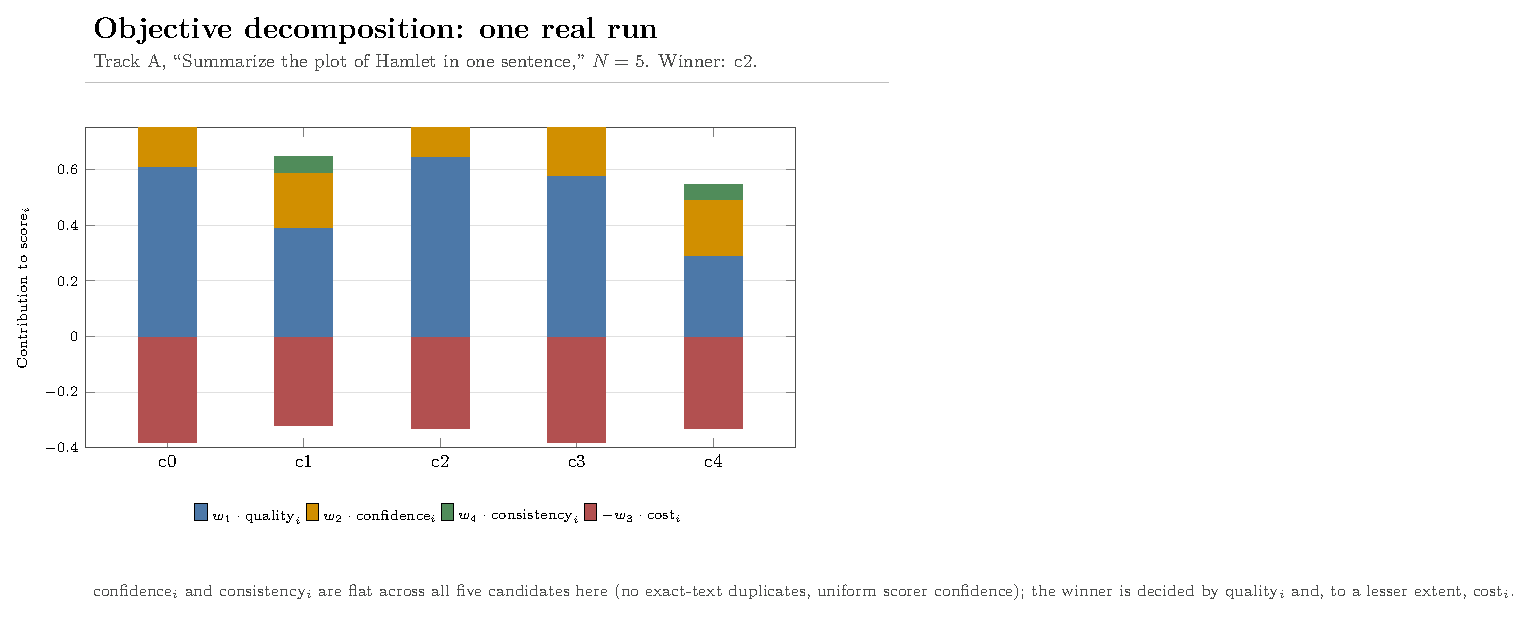
\includegraphics[width=0.85\textwidth]{Figure_3_WorkedExample.pdf}
\caption{The same run as Table~\ref{tab:worked-example}, as stacked weighted
contributions to $\text{score}_i$. Confidence and consistency are constant
across candidates here (no duplicates; uniform scorer confidence), so the
ranking is decided by quality and cost. These candidates are one-sentence
summaries; on multi-hundred-word reasoning outputs the cost term is far
larger relative to quality (Section~\ref{sec:cost-diagnosis}).}
\label{fig:worked-example}
\end{figure}


\begin{figure}[htbp]
\centering
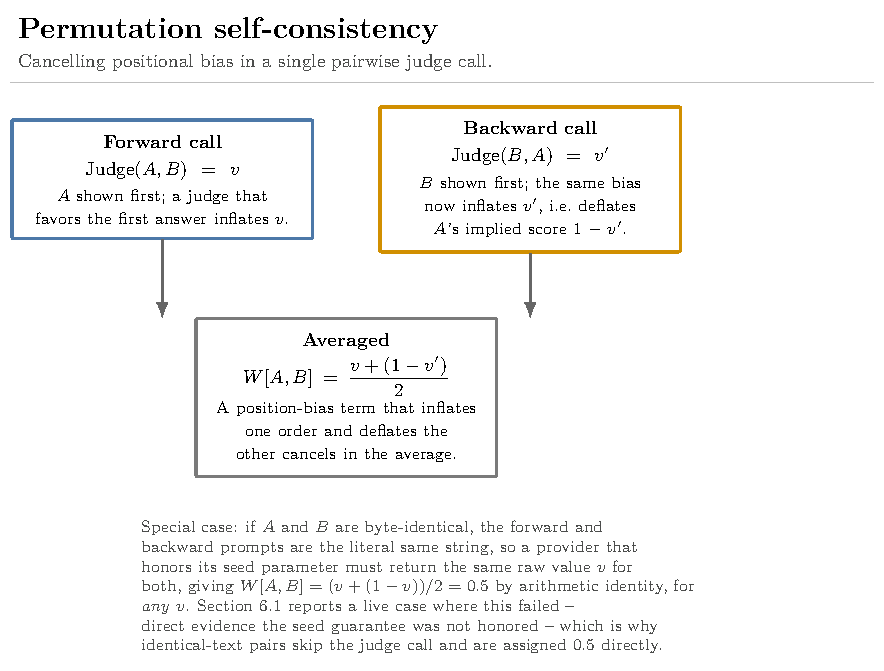
\includegraphics[width=0.85\textwidth]{Figure_2_BiasCancellation.pdf}
\caption{Forward/backward averaging cancels equal additive positional
effects, not arbitrary order dependence. For identical trimmed candidate
texts, the implementation skips both calls and directly assigns $W=0.5$.}
\label{fig:bias-cancel}
\end{figure}

\end{document}
